
\chapter{Pravděpodobnost, statistika a zpracování digitálních obrazú}
\section{Pravděpodobnost}
\subsection{Náhodné jevy, Prostory elementárních jevů, Jevová Pole}
Symbolem $\omega$ budeme značit \textbf{elementární jev}. Elementárním jevem můžeme rozumět např. výsledek pokusu, jenž není jednoznačně určen podmínkami, za kterých se odehrává (Př.: výsledek hodu kostkou). Množinu všech elementáních jevů označujeme $\Omega$ a nazýváme ji \textbf{Prostor elementárních jevů.} (Jevové pole). Většinou se nezajímáme o jednotlivé elementární jevy ale o určité jejich množiny (Př.: Při hodu kostkou padne sudé číslo, atp.). Z matematického hlediska  je výhodné zajímat se o takový systém množin elementárních jevů, který tvoří $\sigma$-algebru.

\begin{definition}
Řekneme, že jev $A$ je elementární jev, jestliže neexistují jevy $B$ a $C$ různé takové, že $A=B\cup C$
\end{definition}

\begin{definition}\label{SihmaAlgebra}(jevová \textbf{$\sigma$-algebra})
Nechť $ \Omega $ je základní prostor přiřazený náhodnímu pokusu a $ 2^{\Omega} $ její potenční množina. Množinu $\mathcal{A} \subseteq 2^{\Omega} $ nazveme jevovou $\sigma$-algebrou, jestliže
\begin{itemize}
\item[\textit{(i)}] $ \Omega \in \mathcal{A} $.
\item[\textit{(ii)}] $\mathcal{A}$ je uzavřená na operaci doplňek, to jest, jestliže $A \in \mathcal{A}$ pak i $ A^{c} \in \mathcal{A} $.
\item[\textit{(iii)}] $\mathcal{A}$ je uzavřená na operaci spočetné sjednocení, to jest, jestliže $ \lbrace A_{n} \rbrace_{n \in \mathbb{N}} \in \mathcal{A}$ potom i $ \bigcup_{n \in \mathbb{N}}A_{n} \in \mathcal{A} $
\end{itemize}
Množina $A\in \mathcal{A} $ se nazývá jev, dvojice $(\Omega,\mathcal{A})$ jevové pole.
\end{definition}

\subsection{Axiomatická pravděpodobnost}

Naším cílem je být schopni jednotlivým množinám patřícím do $\mathcal{A}$ připisovat pravděpodobnost, t.j. chtěli bychom být schopni množiny $\mathcal{A}$ měřit. Pro zadefinování pravěpodobnostní míry budeme potřebovat následující:


\begin{definition}\label{SihmaAditivitaDef}(\textbf{$\sigma$-aditivita})
Nechť $\mathcal{A}\subset 2^{\Omega}$ a nechť $\mu : \mathcal{A} \longrightarrow [0,\infty]$ je množinová funkce. Řekneme že $\mu$ je $\sigma$ aditivní, jestliže pro libovolné $\lbrace A_{n} \rbrace_{n\in \mathbb{N}} \in \mathcal{A} $ vzájemně disjunktní, splňující $\bigcup_{n \in \mathbb{N}}\in \mathcal{A}$ platí 
\begin{equation}\label{SihmaAditivitaRce}\nonumber
\mu \bigg( \bigcup_{n \in \mathbb{N}}A_{n} \bigg) = \sum_{n \in \mathbb{N}} \mu(A_{n})
\end{equation}

\end{definition}

Nyní už můžeme definovat míru a pstní míru.

\begin{definition}\label{MiraPstniMiraDef}(\textbf{ Pravděpodobnostní míra})
Nechť $\mathcal{A} \subset 2^{\Omega}$ je $\sigma$-algebra a nechť $\mu:\mathcal{A} \longrightarrow [0,\infty]$ je množinová funkce splňující $\mu(\emptyset) = 0$. $\mu$ nazveme \textbf{pravděpodobnostní míra}, jestliže $\mu$ je $\sigma$-aditivní, a $\mu(\Omega) = 1$.
V dalším budeme pravděpodobnostní míru označovat $\mathbf{P}$.
\end{definition}

\begin{definition}\label{PstniProstor}\textbf{(Pravděpodobnostní prostor)}
\begin{itemize}
\item[(i)] Dvojice $(\Omega, \mathcal{A})$ tvořený neprázdnou množinou $\Omega$ a $\sigma$-algebrou $\mathcal{A}\subset 2^{\Omega}$ se nazývá měřitelný prostor. Množiny $A \in \mathcal{A}$ se nazývají měřitelné množiny. Jestliže $\Omega$ je nejvýše spočetně nekonečné a jestliže $\mathcal{A} = 2^{\Omega}$, pak nazveme měřitelný prostor $(\Omega, 2^{\Omega})$ diskrétní.
\item[(ii)] Trojice $(\Omega, \mathcal{A}, \mu)$ se nazývá prostor s mírou, jestliže $(\Omega, \mathcal{A})$ měřitelný prostor, a jestliže $\mu$ je $\sigma$-aditivní na $\mathcal{A}$.
\item[(iii)] Jestliže navíc $\mu(\Omega)= 1$ (viz Definici \ref{MiraPstniMiraDef} - Pstní míra), potom $(\Omega, \mathcal{A}, \mu)$ se nazývá pravděpodobnostní prostor. V tomto případě se množiny $A \in \mathcal{A}$ nazývají jevy.
\end{itemize}
\end{definition}

\begin{definition}\textbf{(Konečnost, $\sigma$-konečnost)}
Nechť $\mathcal{A}$ je $\sigma$-algebra. Množinovou funkci $\mu: \mathcal{A} \longrightarrow [0,\infty]$, která je aditivní na $A$ nazveme
\begin{itemize}
\item[(i)] \textbf{konečnou}, jestliže $\mu(A)<\infty$ pro každé $A \in \mathcal{A}$.
\item[(ii)]\textbf{$\sigma$-konečnou}, jestliže existuje posloupnost množin $\Omega_{1},\Omega_{2}, ... \in \mathcal{A}$ takových, že $\Omega = \bigcup_{n=1}^{\infty}\Omega_{n}$ , a  že $\mu(\Omega_{n})<\infty$ pro všechna $n \in \mathbb{N}$.
\end{itemize}
\end{definition}

\subsection{Vlastnosti pravděpodobnosti}\label{SubsVlastnostiPsti}
\begin{theorem} Nechť $(\Omega, \mathcal{A},\textbf{P}$ je pravděpodobnostní prostor. Pak pro libovolné jevy $A,A_1,A_2,\ldots$ má pravděpodobnost následující vlastnosti:
\begin{itemize}
\item[(i)] $\textbf{P}[\emptyset] = 0$.
\item[(ii)] $0 \leq \textbf{P}[A] \leq 1$.
\item[(iii)] Je-li $A_{1} \subseteq A_{2}$, pak $\textbf{P}[A_{1}] \leq \textbf{P}[A_{2}]$.
\item[(iv)] Je-li $A_{1} \subseteq A_{2}$, pak $\textbf{P}[A_{2} - A_{1}] = \textbf{P}[A_{2}] - \textbf{P}[A_{1}]$.
\item[(v)] $\textbf{P}[\overline{A}] = 1 - \textbf{P}[A]$.
\item[(vi)] $\textbf{P}[A_{1} \setminus A_{2}] = \textbf{P}[A_{1}] - \textbf{P}[A_{1} \cap A_{2}].$
\item[(vii)] $\textbf{P}[A_{1} \cup A_{2}] = \textbf{P}[A_{1}] + \textbf{P}[A_{2}] - \textbf{P}[A_{1} \cap A_{2}]$
\item[(viii)] 
\begin{align*}
\textbf{P}\bigg[ \bigcup_{i = 1}^{n} A_{i} \bigg] &= \sum_{i=1}^{n}\textbf{P}[A_{i}] - \sum_{i=1}^{n-1}\sum_{j=i+1}^{n}\textbf{P}[A_{i} \cap A_{j}] \\
&= \sum_{i=1}^{n-2}\sum_{j=i+1}^{n-1}\sum_{k=j+1}^{n}\textbf{P}[A_{i} \cap A_{j} \cap A_{k}]- ... + (-1)^{n-1}\textbf{P}[A_{1} \cap A_{2} \cap ... \cap A_{n}]
\end{align*}
\item[(ix)] $\textbf{P}[\bigcup_{i=1}^{n} A_{i}] \leq \sum_{i=1}^{n} \textbf{P}[A_{i}].$
\end{itemize}
\end{theorem}

\subsection{Podmíněná pravděpodobnost}
\begin{definition}\textbf{(Podmíněná pravděpodobnost)}\label{podm_pst}
Nechť $( \Omega, \mathcal{A}, \textbf{P})$ je pravděpodobnostní prostor a $A \in \mathcal{A}$. Podmíněnou pravděpodobnost  jevu $B$ za podmínky $A$ definujeme pro libovolné $B \in \mathcal{A}$ jako
\begin{equation}
\textbf{P}[B|A] = \frac{\textbf{P}[A \cap B]}{\textbf{P}[A]},
\end{equation}
za předpokladu, že $ \textbf{P}[A] > 0 $.
\end{definition}

Poznámka: \\
Uvažujme pravděpodobnostní prostor $( \Omega, \mathcal{A}, \textbf{P})$. Snadno se vidí, že pro nějaký pevně daný jev $A \in \mathcal{A}$, $\textbf{P}[A] > 0$ podmíněná pravděpodobnost $P[\cdot | A] $ splňuje $\sigma$-aditivitu a je normovaná, t.j. $\textbf{P}[\Omega | A] = 1$ a je tedy také pravděpodobnostní mírou ( = pravděpodobností) ve smyslu Definice \ref{MiraPstniMiraDef}. Důsledkem tohoto má také všechny vlastnosti axiomatické pravděpodobnosti (viz Odstavec \ref{SubsVlastnostiPsti}, nebo Skripta Michálek, str. 30).
\begin{theorem}[Výpočet pravděpodobnosti průniku]
Nechť $(\Omega,\mathcal{A},\textbf{P})$ je pravděpodobnostní prostor, $A_1,A_2,\ldots,A_n \in \mathcal{A}$ jsou takové, že $\textbf{P}(A_1\cup \ldots \cup A_n) > 0$. Pak
\begin{equation*}
\textbf{P}(A_1\cup \ldots \cup A_n) =\textbf{P}(A_1)\textbf{P}(A_2|A_1)\textbf{P}(A_3|A_1\cup A_2)\ldots \textbf{P}(A_n|A_1\cup \ldots \cup A_{n-1})
\end{equation*}
\end{theorem}

\begin{theorem}\label{PodmPSumForm}\textbf{(Sumační formule)/(Vzorec pro výpočet úplné pravděpodobnosti)} Nechť $( \Omega, \mathcal{A}, \textbf{P})$ je pravděpodobnostní prostor a $I$ je spočetná množina a nechť $(B_{i})_{i \in I}$ jsou vzájemně disjunktní množiny s $\textbf{P}[\bigcup_{i \in I}B_{i}] = 1$ (tj. tvoří rozklad množiny $\Omega$). Potom pro libovolné $A \in \mathcal{A}$ máme
\begin{equation}
\textbf{P}[A] = \sum_{i \in I}\textbf{P}[A | B_{i}]\textbf{P}[B_{i}].
\end{equation}
\end{theorem}
\begin{proof}
Díky $\sigma$-aditivitě $\textbf{P}$ máme
\begin{equation}
\textbf{P}[A] = \textbf{P}\bigg[ \bigcup_{i \in I}(A \cap B_{i} \bigg] = \sum_{i\in I} \textbf{P}[A \cap B_{i}] = \sum_{i \in I}\textbf{P}[A|B_{i}]\textbf{P}[B_{i}].
\end{equation}
\end{proof}

\begin{theorem}\label{PodmPBayes}\textbf{(Bayesova formule)}
 Nechť $( \Omega, \mathcal{A}, \textbf{P})$ je pravděpodobnostní prostor a $I$ je spočetná množina a nechť $(B_{i})_{i \in I}$ jsou vzájemně disjunktní množiny s $\textbf{P}[\bigcup_{i \in I}B_{i}] = 1$. Potom pro libovolné $A \in \mathcal{A}$ s $\textbf{P}[A]>0$ a libovolné $k \in I$ máme
\begin{equation}
\textbf{P}[B_{k}|A] = \frac{\textbf{P}[A|B_{k}]\textbf{P}[B_{k}]}{\sum_{i \in I}\textbf{P}[A|B_{i}]\textbf{P}[B_{i}]}.
\end{equation} 
\end{theorem}
\begin{proof}
Máme
\begin{equation}
\textbf{P}[B_{k}|A] = \frac{\textbf{P}[B_{k} \cap A]}{\textbf{P}[A]} = \frac{\textbf{P}[A|B_{k}]\textbf{P}[B_{k}]}{\textbf{P}[A]}.
\end{equation}
Následným využitím výrazu pro $\textbf{P}[A]$ z Věty \ref{PodmPSumForm} je tvrzení dokázáno.
\end{proof}

\subsection{Nezávislost}
\begin{definition}\label{DefJednoduchaNez}\textbf{Nezávislost jevů (Součinové pravidlo)} Nechť $( \Omega, \mathcal{A}, \textbf{P})$ je pravděpodobnostní prostor. Řekneme, že dva jevy $A,B \in \mathcal{A}$ jsou nezávislé, jestliže platí
\begin{equation}
\textbf{P}(A \cap B) = \textbf{P}(A) \cdot \textbf{P}(B).
\end{equation}
Analogicky pro více jevů, nechť $I$ je libovolná indexová množina a $(A_{i})_{i \in I}$ libovolný systém jevů. Tento systém jevů $(A_{i})_{i \in I}$ nazveme nezávislý, jestliže pro libovolnou konečnou podmnožinu $J \subset I$ platí
\begin{equation}
\textbf{P}\bigg[ \bigcap_{j \in J} A_{j} \bigg] = \prod_{j \in J} \textbf{P}[A_{j}].
\end{equation}
\end{definition}

\begin{theorem}
Nechť $( \Omega, \mathcal{A}, \textbf{P})$ je pravděpodobnostní prostor. Pak platí
\begin{enumerate}
\item když $A$ a $B$ jsou nezávislé, pak i $A$ a $\overline{B}$, resp. $\overline{A}$ a $B$, resp. $\overline{A}$ a $\overline{B}$ jsou (ve dvou) nezávislé
\item Jev nemožný a libovolný jev $A$ jsou nezávislé.
\item Jev jistý a libovolný jev $A$ jsou nezávislé
\item Když $0<\textbf{P}(B)<1$ pak platí následující tvrzení: Jevy $A$ a $B$ jsou nezávisé právě tehdy, když $\textbf{P}(A|B)=\textbf{P}(B|A)$
\end{enumerate}
\end{theorem}

\begin{theorem}
Nechť $( \Omega, \mathcal{A}, \textbf{P})$ je pravděpodobnostní prostor a náhodné jevy $A_1,\ldots,A_n \in \mathcal{A}$ jsou skupinově nezávislé. Pak platí
\begin{enumerate}
\item Každá alespoň dvouprvková podmnožina z těchto jevů je skupinově nezávislá.
\item Nahradíme-li $k$ jevů mezi $A_1,A_2,\ldots,A_n$ jejich doplňky, dostáváme $n$-tici skupinově nezávislých jevů
\item $\textbf{P}(\cup_{i-1}^{n} A_i)=1-\prod_{i-1}^{n}(1-P(A_i))$ 
\end{enumerate}
\end{theorem}


\section{Náhodná veličina}
\subsection{Definice}
Pro úplnost (a taky protože to Alčena po mně chtěla) uvedu nejprve konstrukci borelovské $\sigma$-algebry.
\begin{theorem}{(\textbf{O průniku systémů množin})}
Nechť $I$ je libovolná indexová množina, dále předpokládejme, že pro $\forall i \in I$ je $\mathcal{A}_{i}$ $\sigma$-algebra. Potom množina $$\mathcal{A}_{I} = \lbrace A \in 2^{\Omega} : A \in \mathcal{A}_{i} \quad pro \quad \forall i \in I \rbrace = \bigcap_{i \in I} \mathcal{A}_{i}$$ je $\sigma$-algebra. 
\end{theorem}
\begin{proof}
Důkaz spočívá v ukázání, že $\mathcal{A}_{I}$ splňuje vlastnosti $(i) - (iii)$ definice $\sigma$-algebry.
\begin{itemize}
\item[\textbf{(i)}] Zřejmě $\Omega \in \mathcal{A}_{i}$ pro $\forall i \in I$, jelikož $\mathcal{A}_{i}$ je $\sigma$-algebra pro $\forall i \in I$, odtud $\Omega \in \mathcal{A}_{I}$
\item[\textbf{(ii)}] Nechť $A\in \mathcal{A}_{I}$ je libovolná množina, pak $A\in \mathcal{A}_{i}$ pro $\forall i \in I$ , z vlastností $\sigma$-algebry plyne, že $A^{c}\in \mathcal{A}_{i}$ pro $\forall i \in I$, tedy $A^{c}\in \mathcal{A}_{I}$
\item[\textbf{(iii)}] Nechť $A_{1},A_{2}...\in \mathcal{A}_{I}$ jsou libovolné, pak $A_{n}\in \mathcal{A}_{i}$ pro $\forall i \in I$ a pro $\forall n \in \mathbb{N}$ , opět z vlastností $\sigma$-algebry dostáváme, že $ \bigcup_{n \in \mathbb{N}}A_{n} \in \mathcal{A}_{i} $ pro $\forall i \in I$, odtud $\bigcup_{n \in \mathbb{N}}A_{n} \in \mathcal{A}_{I}$.
\end{itemize}
\end{proof}
\begin{theorem}{(\textbf{Generovaná $\sigma$-algebra})}
Nechť $\epsilon \subset 2^{\Omega}$ je libovolné, potom existuje nejmenší $\sigma$-algebra $\sigma(\epsilon)$ obsahující $\epsilon$: $$\sigma(\epsilon) = \bigcap_{\mathcal{A} \quad je \quad \sigma-algebra, \quad \epsilon \subset \mathcal{A}}\mathcal{A}$$ 
$\sigma(\epsilon)$ se nazývá $\sigma$-algebra generovaná $\epsilon$, $\epsilon$ se nazývá generátor.
\end{theorem}
\begin{proof}
Jelikož $\mathcal{A} = 2^{\Omega}$ je $\sigma$-algebra a platí $\epsilon \subset 2^{\Omega}$, $\sigma(\epsilon)$ je neprázdná. Podle předchozí věty $\sigma(\epsilon)$ je $\sigma$-algebra. Je zřejmé, že $\sigma(\epsilon)$ je nejmenší $\sigma$-algebra obsahující $\epsilon$.
\end{proof}


\begin{definition}\textbf{(Topologie)}
Nechť $ \Omega $ je libovolná množina a $ 2^{\Omega} $ její potenční množina. Libovolnou množinu $\tau \subset 2^{\Omega} $ tvořenou pouze otevřenými množinami z $\Omega$ nazveme \textit{topologií}, jestliže splňuje následující vlastnosti:
\begin{itemize}
\item[\textit{(i)}] $ \Omega, \emptyset \in \tau $.
\item[\textit{(ii)}] Jestliže $\lbrace O_{n} \rbrace_{n \in \mathbb{N}} \in \tau$ je posloupnost otevřených množin náležící do $ \tau$, potom $\bigcup_{n \in \mathbb{N}}O_{n} \in \tau$.
\item[\textit{(iii)}] Jestliže $O_{1}, ..., O_{n} \in \tau $ jsou otevřené množiny náležící do $\tau$ potom $O_{1}\cap ...\cap O_{n} \in \tau$.
\end{itemize}
Dvojici $(\Omega, \tau)$ potom nazýváme \textit{topologický prostor}.
\end{definition}


\begin{definition}[\textbf{(Borelovská $\sigma$-algebra)}]
Nechť $(\Omega, \tau)$ je topologický prostor. Potom $\sigma$-algebra $$\mathcal{B}(\Omega)=\mathcal{B}(\Omega,\tau) = \sigma(\tau),$$ nejmenší $\sigma$-algebra generovaná topologií $\tau$, se nazývá \textbf{Borelovská} $\bm{\sigma}$ \textbf{algebra}. Její prvky $A \in \mathcal{B}(\Omega, \tau)$ se nazývají \textbf{Borelovské množiny}, nebo \textbf{Borelovské měřitelné množiny}.
\end{definition}

Představme si, že máme náhodný experiment - hod kostkou. Možné jevy jsou: "padne jednička", "padne dvojka", ... atd. Pro další zkoumání našeho experimentu bychom chtěli jednotlivým jevům přiřadit nějaké číselné ohodnocení, takovýto model by nám například umožnil výpočet číselných charakteristik jako jsou střední hodnota, rozptyl atd. Naším cílem je tedy přiřadit např. jevu "padne dvojka" číslo $2$, tedy "padne dvojka" $\longrightarrow 2$. Definujme náhodnou veličinu.
\begin{definition}{(\textbf{Náhodná veličina})}
Nechť $( \Omega, \mathcal{A}, \textbf{P}) $ je pravděpodobnostní prostor, nechť $(\mathbb{R}, \mathcal{B})$ je reálná osa a systém jejích Borelovských množin, potom měřitelné zobrazení $X: (\Omega, \mathcal{A}, \textbf{P}) \longrightarrow (\mathbb{R}, \mathcal{B}) $ nazveme náhodná veličina.
\end{definition}

Každé Borelovské možine lze přiřadit její vzor $X^{-1}(B) = \lbrace \omega \in \Omega : X(\omega) \in B \rbrace$ s pomocí $X$ (náhodná veličina je měř. zobrazení) a pravděpodobnostní míru $Q(B) = \textbf{P}\lbrace X^{-1}(B) \rbrace$.



\subsection{Distribuční funkce}
\begin{definition}{\textbf{(Rozdělení, distribuční funkce)}}
Nechť $X$ je náhodná veličina
\begin{itemize}
\item[(i)] pravděpodobnostní míru $\textbf{P}_{X} = \textbf{P} \circ X^{-1}$ nazveme zákonem rozdělení (rozdělením) náhodné veličiny $X$. Když $\textbf{P}_{X} = \mathcal{L}$ píšeme $X \sim \mathcal{L}$ a říkáme, že $X$ má rozdělení $\mathcal{L}$.
\item[(ii)] zobrazení $F_{X}: x \mapsto \textbf{P}\lbrace X < x \rbrace$ se nazývá distribuční funkce náhodné veličiny $X$.
\end{itemize}
\end{definition}
\begin{remark}
Distribuční funkce přiřazuje každému $x \in \mathbb{R}$ pomocí $X$ pravděpodobnostní míru Borelovské možiny $B = ( -\infty, x)$. 

Mezi zákonem rozdělení a distribuční funkcí je vzájemně jednoznačný vztah.
\end{remark}
\begin{remark}{\textbf{(Vlastnosti distribuční funkce)}}
Každá distribuční funkce je neklesající, zleva spojitá (zprava pokud do definičního vztahu zaměním $\leq$ za $<$), může mít jen spočetně mnoho bodů nespojitosti a platí pro ni
\begin{itemize}
\item[(i)] $\lim_{x \longrightarrow -\infty}F_{X} = 0$ a $\lim_{x \longrightarrow \infty}F_{X} = 1$.
\item[(ii)]pro libovolná reálná $x_{1}, x_{2}$ taková že $x_{1} < x_{2}$ $\textbf{P}(x_{1} < X \leq x_{2}) = F(x_{2}) - F(x_{1})$
\end{itemize} 
\end{remark}

\subsection{Diskrétní a spojité náhodné veličiny}
V matematické statistice mají největší uplatnění následující dva typy distribučních funkcí:
\begin{itemize}
\item[(a)] Distribuční funkce je funkce skoků. Potom říkáme, že má náhodná veličina $X$ diskrétní rozdělení pravděpodobnosti. Jak již bylo zmíněno, bodů nespojitosti může být jen spočetně mnoho, označme je $x_{1}, x_{2}, ...$. Nechť $p_{k}$ je velikost skoku funkce $F_{X}$ v bodě $x_{k}$. Lze ukázat, že platí $p_{k} = \textbf{P}\lbrace X = x_{k} \rbrace$.
\item[(b)] Existuje taková funkce $f(x), $ že platí
\begin{equation}\label{VyjadreniDistFce}
F(x) = \int_{-\infty}^{x}f(t)dt.
\end{equation}
\end{itemize}
Pak se jedná o spojité rozdělení pravěpodobnosti. Z teorie míry je známo, že $F_{X}$ má vyjádření \eqref{VyjadreniDistFce} právě tehdy, když je absolutně spojitá (viz Radonova-Nikodymova věta). Protože $F_{X}$ je neklesající, musí platit $f(x) \geq 0$ skoro všude. Je-li třeba, hustota se upraví tak, aby byla všude nezáporná. Pod pojmem hustoty budeme rozumět jen její nezápornou verzi.
\subsection{Číselné charakteristiky}
Pro zavedení číselných charakteristik náhodných veličin budeme potřebovat připomenout některé pojmy z funkcionální analýzy. Nechť $f : (\Omega, \mathcal{A}, \textbf{P}) \longrightarrow (\mathbb{R}, \mathcal{B})$ je zobrazení, nechť $p \in \mathbb{N}$, zobrazení $f$ nazveme $p$-integrovatelné, jestliže
\begin{equation}
\bigg(\int_{\Omega}|f|^{p} d\textbf{P}\bigg)^{\frac{1}{p}} < \infty.
\end{equation}
Symbolem $\mathcal{L}^{p}(\textbf{P})$ označíme množinu všech zobrazení, která jsou $p$-integrovatelná vzhledem k míře $\textbf{P}$. Speciálně, pokud $p = 1$ říkáme, že je $f$ integrovatelné.

V následující definici zavedeme pojmy střední hodnota a rozptyl, intuitivně pod pojmem střední hodnota rozumíme "průměrný" výsledek pokusu po nekonečně mnoha opakováních. Rozptylem potom rozumíme střední hodnotu kvadrátu vzdáleností hodnot náhoné veličiny od její střední hodnoty.
\begin{definition}{(\textbf{Střední hodnota, momenty, rozptyl}}
Nechť $X$ je integrovatelná náhodná veličina, potom interál
\begin{equation}
\textbf{E}X = \int_{\Omega}X(\omega) d\textbf{P}(\omega)
\end{equation} 
nazveme střední hodnota $X$.

Nechť navíc $X \in \mathcal{L}^{p}$ potom 
\begin{equation}
\mu'_{k}=\textbf{E}X^{k}=\int_{\Omega}X^{k}(\omega) d\textbf{P}(\omega) 
\end{equation}
nazýváme obecný moment $k$-tého řádu náhodné veličiny $X$ a 
\begin{equation}
\mu_{k} = \mathbf{E}[X - \mathbf{E}X]^{k}
\end{equation}
centrální moment $k$-tého řádu náhodné veličiny $X$.

Pro $k = 2$ značíme $\mathbf{var}X = \mathbf{E}[X - \mathbf{E}X]^{2} = \mathbf{E}X^{2} - (\mathbf{E}X)^{2}$ a nazýváme rozptyl náhodné veličiny $X$.
\end{definition}
\begin{remark}
V případě pravděpodobnostní míry (a konečné míry obecně) jsou prostory $\mathcal{L}^{p}$ uspořádané následujícím způsobem. Pokud $p > q$ potom $\mathcal{L}^{p} \subseteq \mathcal{L}^{q}$. Odtud zřejmě plyne, že pokud pro $X$ existuje moment $k$-tého řádu, potom nutně musí existovat i momenty všech nižších řádů.
\end{remark}
\begin{remark}
Obvykle bývá známa jenom distribuční funkce, většinou se proto konkrétní výpočet provádí podle vzorce (viz Větu o přenosu integrace, třeba v Andělovi) 
\begin{equation}
\mathbf{E}X = \int_{\mathbb{R}}xdF(x),
\end{equation}
což, za předpokladu, že existuje hustota můžeme přepsat na
\begin{equation}
\mathbf{E}X = \int_{\mathbb{R}}tf(t)dt
\end{equation}
a pro náhodnou veličinu s diskrétním rozdělením pravděpodobnosti
\begin{equation}
\sum_{i: x_{i}\in B}x_{i}p_{i}.
\end{equation}
\end{remark}

\begin{theorem}{\textbf{(Vlastnosti střední hodnoty)}}
Nechť $X$ je integrovatelná náhodná veličina a $a, B \in \mathbb{R}$ jsou konstanty, potom platí
\begin{equation}
\mathbf{E}[a + BX] = a + B\mathbf{E}X.
\end{equation}
\end{theorem}
\begin{proof}
Střední hodnota je zřejmě lineární operátor, tvrzení je toho důsledkem.
\end{proof}

\begin{theorem}{\textbf{(Vlastnosti rozptylu)}}
Nechť $X$ je kvadraticky integrovatelná náhodná veličina a $a, B \in \mathbb{R}$ jsou konstanty, potom platí
\begin{equation}
\mathbf{var}[a + BX] = B^{2}\mathbf{var}X
\end{equation}
\end{theorem}
\begin{proof}
V důkazu se využije linearity střední hodnoty:
\begin{align*}
\mathbf{var}[a + BX] &= \mathbf{E}[a + BX]^{2} - (\mathbf{E}[a + BX])^{2} \\
&= \mathbf{E}[a^{2} + 2aBX + B^{2}X^{2}] - a^{2} - 2aB\mathbf{E}X - B^{2}(\mathbf{E}X)^{2} \\
&= B^{2}\mathbf{E}X^{2} - B^{2}(\mathbf{E}X)^{2} \\
&= B^{2}\mathbf{var}X
\end{align*}
\end{proof}

\subsection{Kvantily}
\begin{figure}[h]
\begin{center}
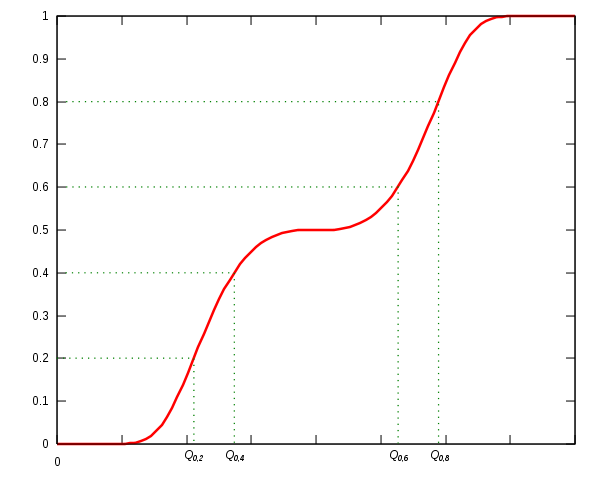
\includegraphics[scale=0.5]{Obrazky/600px-Quantile.png}
\caption{Obrázek z wiki :D, x-ová osa: kvantily, y-ová osa: hodnoty pravděpodobnosti}
\end{center}
\end{figure}
V následujícím zavedeme pojem kvantilu. Kvantil je míra polohy popisující body, ve kterých distribuční funkce náhodné veličiny prochází danou hodnotou, tedy např.: kvantil $F^{-1}(0.5)$ dává hodnotu z definičního oboru distribuční funkce $F$, ve které poprvé nabyde hodnoty $0.5$.
\begin{definition}
Nechť $F$ je distribuční funkce. Zaveďmě funkci $F^{-1}$ předpisem
\begin{equation}
F^{-1}(u) = \inf\lbrace x : F(x) \geq u \rbrace, \enskip 0 < u < 1.
\end{equation}
Pak se funkci $F^{-1}$ nazývá kvantilová funkce odpovídající distribuční funkci $F$, hodnotám $F^{-1}(u)$ se říká kvantily.
\end{definition}

\begin{remark}
Je li $F$ striktně rostoucí, potom je $F^{-1}$ inverzní funkce k $F$.
\end{remark}

\begin{remark}
$Q_{0.5} = F^{-1}(0.5)$ se nazývá medián. Kvantily $Q_{0.25} = F^{-1}(0.25)$, $Q_{0.75} = F^{-1}(0.75)$ se nazývají dolní a horní kvartil.
\end{remark}
\subsection{Charakteristická funkce}
\begin{definition}
Charakteristickou funkci $\psi(t)$ náhodné veličiny $X$ definujeme vzorcem
\begin{equation}
\psi(t) = \mathbf{E}e^{itX} = \mathbf{E}\cos(tX) + i\mathbf{E}\sin(tX), \enskip t \in \mathbb{R}.
\end{equation}
\end{definition}

\begin{remark}
Má-li náhodná veličina $X$ distribuční funkci $F$, pak můžeme psát $\psi(t) = \int e^{itx}dF(x)$ (viz Větu o přenosu integrace v Andělovi). Platí, že $\psi$ je stejnoměrně spojitá, $\psi(0) = 1$ a $|\psi(t)| \leq 1$.
\end{remark}

Charakteristickou funkci lze využít k výpočtu obecných momentů, pokud existují.
\begin{theorem}
Existují-li konečné momenty $\mu_{1}', ..., \mu_{n}',$ pak charakteristická funkce $\psi$ má prvních $n$ derivací a platí
\begin{equation}
\psi^{(k)}(0) = i^{k}\mu_{k}' \enskip k = 1, ..., n, \enskip \psi(t) = \sum_{k = 0}^{n}\mu_{k}' \frac{(it)^{k}}{k!} + O(t^{n}), \enskip t \longrightarrow 0.
\end{equation}
\end{theorem}
\begin{proof}
Viz Rényi (1972).
\end{proof}

Pro zajímavost uveďme následující tvrzení popisující závislost charakteristické funkce a distribuční funkce n. v. $X$.
\begin{theorem}
Nechť $\psi$ je charakteristická finkce odpovídající distribuční funkci $F$ a nechť $a, b (a < b)$ jsou body spojitosti funkce $F$. Pak platí
\begin{equation}
F(b) - F(a)  = \frac{1}{2\pi} \int_{-\infty}^{\infty}\bigg[ \psi(t) \frac{e^{-ita}-e^{-itb}}{2it} - \psi(-t)\frac{e^{ita}-e^{itb}}{2it} \bigg] dt.
\end{equation}
\end{theorem}
\begin{proof}
Viz Renyi (1972).
\end{proof}
Odtud plyne, že distribuční funkce je charakteristickou funkcí jednoznačně určena.

%Uvažujme posloupnost distribučních funkcí $\lbrace F_{n} \rbrace$ a distribuční funkci $F$. Jestliže $F_{n}(x) \longrightarrow F(x)$ v každém bodě $x$, který he bodem spojitosti funkce $F$, pak říkáme, že posloupnost $\lbrace F_{n} \rbrace$ slabě konverguje k $F$. Jestliže distribuční funkce náhodných veličin $\lbrace X_{n} \rbrace$ slabě konvergují k distribuční funkci veličiny $X$, pak píšeme $\mathcal{L}(X_{n}) \longrightarrow \mathcal{X}, nebo také $X_{n} \longrightarrow^{d} X $a říkáme, že veličiny $X_{n}$ konvergují v distribuci k $X$.
\subsection{Základní diskrétní rozdělení pravděpodobnosti}
Uveďme příklady diskrétních rozdělení pravděpodobnosti, v poznámkách bude uveden jejich praktický význam, druh pokusu který modelují, atp.
\begin{definition}{\textbf{(Binomické rozdělení}}
Buď $n$ přirozené číslo a $p \in (0, 1)$. Předpokládejme, že $X$ nabývá pouze hodnot $0, 1, ..., n$ a to s pravděpodobnostmi
\begin{equation}
\textbf{P}(X = k) = \binom{n}{k}p^{k}(1-p)^{n-k}, \enskip k = 0, 1, ..., n.
\end{equation}
Pak říkáme, že $X$ má binomické rozdělení a píšeme $X \sim Bi(n,p)$.
\end{definition}
\begin{proposition}
Nechť  $X \sim Bi(n,p)$. potom $\mathbf{E}X = np$, $\mathbf{var}X = np(1-p)$ a $\psi(t) = (1-p + pe^{it})^{n}$.
\end{proposition}
\begin{proof}
Důkaz se mi nechce dělat, ukáže se to tak, že se nějakými manipulacemi s nekonečnou řadou vyjadřující střední hodnotu získá její součet, rozptyl podobně. Char fce. z definice
\end{proof}

\begin{remark}
Binomické rozdělení je diskrétní rozdělení pravděpodobnosti počtu úspěšných pokusů v posloupnosti $n$ nezávislých pokusů.
Modeluje počet úspěchů ve výběru velikosti $n$ z populace o velikosti $N$ s vracením. Př.: Mám osudí s bílými a černými míčky $n$-krát vytáhnu z osudí míček, poznamenám si barvu a vrátím ho zpět, bin. rozd. udává pravděpodobnost že $k$ míčků bude černých (resp. bílých). Pro $n = 1$ se jedná o tzv alternativní rozdělení.
\end{remark}

\begin{definition}{\textbf{(Hypergeometrické rozdělení)}}
Nechť $N, A$ a $n$ jsou přirozená čísla, přičemž $A < N, n < N$. Nechť $X$ nabývá pouze celočíselných hodnot s pravděpodobnostmi 
\begin{equation}
\textbf{P}(X = x)= \frac{\binom{A}{k}\binom{N-A}{n-k}}{\binom{N}{n}} \enskip pro \enskip \max(0, A + n -N)\leq k \leq \min(A, n).
\end{equation}
Pak říkáme, že $X$ má hypergeometrické rozdělení a píšeme $X \sim Hg(N,A,n)$.
\end{definition}
\begin{proposition}
Nechť $X$ má hypergeometrické rozdělení s parametry $N, A$ a $n$, přičemž $A < N, n < N$.  Je-li $N > 1,$ pak 
\begin{equation}
\mathbf{E}X = \frac{nA}{N}, \enskip \mathbf{var}X = \frac{nA(N-A)}{N^{2}}\bigg( 1 - \frac{n-1}{N-1}\bigg).
\end{equation}
\end{proposition}
\begin{proof}
Důkaz je ponechán pro zvídavého čtenáře, jenž je laskavě odkázán, na literaturu zabývající se pravděpodobností a statistikou.
\end{proof}

\begin{remark}
Poznamenejme, že hypergeometrické rozdělení modeluje pravděpodobnost počtu úspěchů ve výběru velikosti $n$ z populace o velikosti $N$ za předpokladu, že výběr probíhá bez opakování. V případě osudí s míčky z příkladu u binomického rozdělení bychom míčky po vytažení již nevraceli zpět.
\end{remark}

\begin{definition}{\textbf{(Poissonovo rozdělení)}}
Nechť $X$ nabývá pouze hodnot $0, 1, ..., $ a to s pravděpodobnostmi 
\begin{equation}
\textbf{P}(X = k) = \frac{\lambda^{k}}{k!}e^{-\lambda},\enskip k = 0, 1, ...,
\end{equation}
kde $\lambda >0$ je dané číslo. Pak říkáme, že $X$ má Poissonovo rozdělení s parametrem $\lambda$ a píšeme $X \sim Po(\lambda)$.
\end{definition}

\begin{proposition}
Nechť $X \sim Po(\lambda)$. Potom $\mathbf{E}X = \lambda,$ $\mathbf{var}X = \lambda$ a $\psi(t) = e^{\lambda(e^{it}-1)}$.
\end{proposition}
\begin{proof}
Důkaz prvních dvou je z definice manipulací s nekonečnými řadami pro získání jejich součtu, třetí z definice char. fce. Toto mám dokonce naTeXované, ale dávat to sem nebudu, anžto je to delší. Kdyby to někoho hrozně strašně moc zajímalo, nechť se zeptá.
\end{proof}
\begin{remark}
Popisuje pravděpodobnost nastání daného počtu nezávislých jevů v určitém časovém intervalu. Například pravděpodobnost obdržení určitého počtu spamových emailů za týden, za předpokladu, že každý email je na všech ostatních nezávislý.
\end{remark}

\subsection{Spojitá rozdělení pravděpodobnosti}
\begin{definition}{\textbf{(Normální rozdělení)}}
Nechť $ \mu \in \mathbb{R}$ a $\sigma > 0$ jsou dané konstanty (parametry). Normální rozdělení je určeno hustotou
\begin{equation}
f(x) = \frac{1}{\sqrt{2\pi}\sigma}\exp \bigg[ -\frac{(x - \mu)^{2}}{2\sigma^{2}} \bigg]
\end{equation}
a označuje se symbolem $N(\mu, \sigma^{2}).$ V případě, že $\mu = 0$ a $\sigma = 1$ nazýváme $N(0, 1)$ standardní normální rozdělení, jeho hustotu značíme $\phi$ a příslušnou distribuční funkci $\Phi$, máme tedy
\begin{equation}
\phi(x) = \frac{1}{\sqrt{2\pi}}e^{\frac{-x^{2}}{2}}, \enskip \Phi(x) = \int_{-\infty}^{x}\phi(t)dt.
\end{equation}
\end{definition}

\begin{proposition}
Nechť $X \sim N(\mu, \sigma^{2})$ potom $\mathbf{E}X = \mu$, $\mathbf{var}X = \sigma^{2}$, šikmost $\alpha_{3} = 0$ a špičatost $\alpha_{4} = 3$. Charakteristická funkce normálního rozdělení má tvar 
\begin{equation}
\psi(t) = \exp\bigg[ i\mu t - \frac{1}{2}\sigma^{2}t^{2} \bigg].
\end{equation}
\end{proposition}
\begin{proof}
Přímým výpočtem.
\end{proof}

\begin{remark}
Normální rozdělení má v matematické statistice a stochastické analýze veliký význam, mnoho statistických modelů je založeno na předpokladu normálního rozdělení. Příkladem je třeba regrese, kde se předpokládá normální rozdělení závisle proměnných, aby bylo možné odvodit intervaly spolehlivosti, nebo testy vycházející z regresní analýzy, např. analýza rozptylu. V této souvislosti připomeňme také centrální limitní větu, která říká, že průměry z výběrů z nezávislých rozdělení konvergují v distribuci k normálnímu rozdělení.
\end{remark}

\begin{definition}{\textbf{(Weibullovo rozdělení)}}
Nechť $c > 0, \enskip p > 0$. Weibullovi rozdělení $W(c, p)$ má hustotu
\begin{equation}
f(x) = cpx^{p-1}\exp[-cx^{p}], \enskip x > 0.
\end{equation}
Pro volbu $p = 1$ získáme exponenciální rozdělení.
\end{definition}

\begin{proposition}
Nechť $X \sim W(c, p)$, platí
\begin{equation}
\mathbf{E}X = \Gamma\bigg( \frac{p + 1}{p} \bigg) c^{-1/p}, \enskip \mathbf{var}X = \bigg[ \Gamma \bigg( \frac{p+2}{p}\bigg) - \Gamma^{2} \bigg( \frac{p + 1}{p}\bigg) \bigg] c^{-2/p}, 
\end{equation}
kde $\Gamma$ je gamma funkce definovaná pro $a>0$ předpisem $\Gamma(a) = \int_{0}^{\infty} x^{a - 1}e^{-x}dx.$
\end{proposition}

\begin{remark}
Weibullovo rozdělení se využívá ve spolehlivosti při modelování životnosti. Dobře vystihuje dobu do poruchy stárnoucího objektu.
\end{remark}

\section{Náhodný vektor}
\subsection{Definice}
Pro zavedení teorie týkající se náhodných vektorů využijeme poznatků a intuice popsané již při zavádění náhodných veličin.
\begin{definition}{\textbf{(Náhodný vektor)}}
Nechť náhodné veličiny $X_{1}, ..., X_{n}$ jsou definovány na témž pravděpodobnostním prostoru $(\Omega, \mathcal{A}, \textbf{P})$. Pak vektor $\textbf{X} = (X_{1}, ..., X_{n})^{T}$ nazveme náhodným vektorem. 
\end{definition}
\begin{theorem}
Náhodný vektor $\textbf{X}$ je měřitelné zobrazení z pravděpodobnostního prostoru $(\Omega, \mathcal{A}, \textbf{P})$ do $(\mathbb{R}_{n}, \mathcal{B}_{n})$.
\end{theorem}
\begin{proof}
Viz Anděl.
\end{proof}
\subsection{Simultální distribuční funkce, diskrétní a spojitý n. v.}
\begin{definition}{\textbf{(Sdružená (simultální) distribuční funkce)}}
Sdruženou distribučná funkci náhodných veličin $X_{1}, ..., X_{n}$ definovaných na témže pravděpodobnostním prostoru $(\Omega, \mathcal{A}, \textbf{P})$ definujeme vzorcem
\begin{equation}
F(x_{1}, ..., x_{n}) = \textbf{P}(X_{1} < x_{1}, ..., X_{n} < x_{n}).
\end{equation}
\end{definition}

Distribuční funkci odpovídá míra $\textbf{P}_{\textbf{X}}$ indukovaná na $(\mathbb{R}_{n}, \mathcal{B}_{n})$ zobrazením $\textbf{X}$, kterou nazýváme sdružené rozdělení veličin $X_{1}, ..., X_{n}$ (viz definici rozdělení).

Existuje-li taková měřitelná funkce $f$, že platí 
\begin{equation}
F(x_{1}, ..., x_{n}) = \int_{-\infty}^{x_{1}}...\int_{-\infty}^{x_{n}} f(u_{1}, ..., u_{n})du_{1}...du_{n},
\end{equation}
říkáme funkci $f$ sdružená (simultální) hustota. Existuje-li hustota, má $F$ skoro všude derivaci a platí
\begin{equation}
\frac{\partial^{n}F(x_{1}, ..., x_{n})}{\partial x_{1}...\partial x_{n}} = f(x_{1}, ..., x_{n}), \enskip s. v.,
\end{equation}
náhodný vektor $X$ potom nazýváme \textbf{spojitý}.

$\textbf{X}$ nazýváme \textbf{diskrétní} náhodný vektor právě tehdy, když existuje nejvýše spočetná množina $M \subset \mathbb{R}^{n}, \enskip M = M_{1} \times ... \times M_{n}$ taková, že $\textbf{P}(\textbf{X} \in M) = 1$.

Opět můžeme definovat pravděpodobností funkci jako
\begin{equation}
p(\textbf{x}) = \textbf{P}(\textbf{X} = \textbf{x}) = \textbf{P}(X_{1} = x_{1}, ..., X_{n} = x_{n} )
\end{equation}
\subsection{Marginální a podmíněné rozdělení}
\begin{definition}{\textbf{(Marginální rozdělení)}}
Nechť $k_{1}, ..., k_{r}$ jsou různá celá čísla taková, že $1 \leq k_{i} \leq n$ pro $i = 1, ..., r$, přičemž $1 \leq r < n.$ Rozdělení náhodného vektoru $(X_{k_{1}}, ..., X_{k_{r}})^{T}$ se nazývá marginální. 
\end{definition}
\begin{example}{\textbf{(Marginální distribuční funkce)}}
Nechť $\textbf{X} = (X_{1}, ..., X_{n})$ je náhodný vektor. Marginální distribuční funkce $G$ veličin $X_{1}, ... X_{k}$, pro $1 \leq k < n$ je dána vzorcem
\begin{equation}
G(x_{1}, ..., x_{k}) = \lim_{\substack{x_{k+1} \longrightarrow \infty \\ ... \\ x_{n} \longrightarrow \infty}} F(x_{1}, ..., x_{k}, x_{k + 1}, ..., x_{n}).
\end{equation}
\end{example}

\begin{remark}
Existuje-li sdružená hustota, pak existují i marginální hustoty, obrácené tvrzení však neplatí.
\end{remark}

Při popisu podmíněného rozdělení se omezíme jen na uvedení vzorců  pro podmíněnou pravděpodobnostní funkci a hustotu diskrétní nebo spojité náhodné veličiny $X$ za podmínky $Y = y$. Obecně to však není tak jednoduché.


Nechť $p(x,y)$ je simultánní pravděpodobnostní funkce diskrétního náhodného vektoru $\textbf{Z} = (X, Y)^{T}$ Pro pravděpodobnostní funkci n.v. $X$ za podmínky $Y = y$ máme 
\begin{equation}
p(x|y) = \frac{p(x,y)}{p(y)}, \enskip pokud \enskip p(y) \neq 0
\end{equation}
kde $p(y)$ je příslušná marginální pravděpodobnostní funkce.

Nechť $f(x,y)$ je sdružená hustota spojitého náhodného vektoru vektoru $\textbf{Z} = (X, Y)^{T}$ Pro hustotu n.v. $X$ za podmínky $Y = y$ máme 
\begin{equation}
f(x|y) = \frac{f(x,y)}{f(y)}, \enskip pokud \enskip f(y) \neq 0
\end{equation}
kde $f(y)$ je příslušná marginální hustota.

\subsection{Nezávislost}
\begin{definition}{\textbf{(Nezávislé náhodné veličiny)}}
Náhodné veličiny $X_{1}, ..., X_{n}$ se nazývají nezávislé, platí-li pro libovolné borelovské množiny vztah
\begin{equation}
\textbf{P}[\cap_{k=1}^{n}\lbrace \omega : X_{k}(\omega) \in B_{k}\rbrace] = \prod_{k = 1}^{n} \textbf{P}\lbrace \omega : X_{k}(\omega) \in B_{k} \rbrace.
\end{equation}
\end{definition}

Z definice je nezávislost náhodných veličin ověřit, uveďme proto formou vět následující kritéria.
\begin{theorem}\label{Kriterium1}
Nechť $\textbf{X}$ má sdruženou distribuční funkci $F$ a nechť $F_{i}$ je marginální distribuční funkce veličiny $X_{i}$, $i = 1, ..., n$. Pak $X_{1}, ..., X_{n}$ jsou nezávislé právě tehdy, když platí $F(x_{1}, ..., x_{n}) = F_{1}(x_{1})\cdot ... \cdot F_{n}(x_{n})$ pro všechna $x_{1}, ..., x_{n}$.
\end{theorem}
\begin{proof}
Viz Renyi (1972).
\end{proof}

Borelovsky měřitelná funkce náhodné veličiny je opět náhodná veličina, funkce nezávislých náhodných veličin jsou také nezávislé. Pro spojité náhodné veličiny máme potom jako důsledek předchozí věty nádlesující tvrzení.
\begin{theorem}
Nechť náhodné veličiny $X_{1}, ..., X_{n}$ mají sdruženou hustotu $f$ a marginální hustoty $f_{1}, ..., f_{n}$. Pak $X_{1}, ..., X_{n}$ jsou nezávislé tehdy a jen tehdy, platí-li
\begin{equation}
f(x_{1}, ..., x_{n}) = f_{1}(x_{1})\cdot ... \cdot f_{n}(x_{n}) \enskip s. \enskip v.
\end{equation}
\end{theorem}
\begin{proof}
Tvrzení je důsledkem Věty \ref{Kriterium1}.
\end{proof}

Pro diskrétní náhodné veličiny máme potom jako důsledek předchozí věty následující tvrzení.
\begin{theorem}
Nechť $X_{1}, ..., X_{n}$ jsou veličiny s diskrétním rozdělením pravděpodobnosti $\mathcal{L}(M_{i}, p_{i})$, mají sdruženou pravděpodobnostní funkci $p$ a marginální pravděpodobnostní funkce $p_{1}, ..., p_{n}$. Pak $X_{1}, ..., X_{n}$ jsou nezávislé tehdy a jen tehdy, platí-li
\begin{equation}
p(x_{1}, ..., x_{n}) = p_{1}(x_{1})\cdot ... \cdot p_{n}(x_{n}) \enskip s. \enskip v.
\end{equation}
\end{theorem}
\begin{proof}
Tvrzení je důsledkem Věty \ref{Kriterium1}.
\end{proof}

\begin{theorem}\label{VetaSeStrHod}
Nechť $X_{1}, ..., X_{n} \in \mathcal{L}^{1}(\Omega)$, pak platí $X_{1}, ..., X_{n}$ jsou nezávislé právě tehdy, když
\begin{equation}
\mathbf{E}(X_{1}, ..., X_{n}) = (\mathbf{E}X_{1}) \cdot ... \cdot (\mathbf{E}X_{n}) 
\end{equation}
\end{theorem}
\begin{proof}
\begin{align*}
\mathbf{E}(X_{1}, ..., X_{n})&= \int ... \int x_{1}...x_{n}dF(x_{1}, ..., x_{n}) \\
&= \int ... \int x_{1}...x_{n}dF(x_{1})...dF(x_{n}) \\
&= \bigg[ \int x_{1}dF(x_{1}) \bigg]...\bigg[ \int x_{n}dF(x_{n}) \bigg]\\ 
&= (\mathbf{E}X_{1})  ... (\mathbf{E}X_{n}),
\end{align*}
kde druhá rovnost je důsledkem Věty \ref{Kriterium1} a třetí je vlastnost L-S integrálu.
\end{proof}

\begin{remark}
Podobná tvrzení lze odovodit pro střední hodnoty a charakteristické funkce.
\end{remark}

\subsection{Číselné charakteristiky}
\begin{definition}{\textbf{(Střední hodnota náhodného vektoru)}}
Nechť $\textbf{X} = (X_{1}, ..., X_{n})^{T}$ je náhodný vektor. Jsou-li náhodné veličiny $X_{i}$, $i = 1, ..., n$ integrovatelné potom definujeme střední hodnotu vektoru $\textbf{X}$ jako
\begin{equation}
\mathbf{E}\textbf{X} = (\mathbf{E}X_{1}, ..., \mathbf{E}X_{n})^{T}.
\end{equation}
\end{definition}

Analogicky se definuje i střední hodnota matice, jejímiž vstupy jsou náhodné veličiny.

\begin{definition}{\textbf{(Kovariance náhodného vektoru)}}
Nechť $\textbf{X} = (X_{1}, ..., X_{n})^{T}$ je náhodný vektor. Jsou-li náhodné veličiny $X_{i}$, $i = 1, ..., n$, kvadraticky integrovatelné, t.j. $\mathbf{E}X_{i} < \infty$ pro $i = 1, ..., n$ pak definujeme kovarianci $\mathbf{cov}(X_{i}, X_{j})$ vztahem
\begin{equation}
\mathbf{cov}(X_{i}, X_{j}) = \mathbf{E}[(X_{i} - \mathbf{E}X_{i})(X_{j} - \mathbf{E}X_{j})] 
\end{equation}
\end{definition}

\begin{proposition}
Nechť $\textbf{X} = (X_{1}, ..., X_{n})^{T}$ je náhodný vektor. Jsou-li náhodné veličiny $X_{i}$, $i = 1, ..., n$, kvadraticky integrovatelné, potom pro kovarianci $X_{i}, X_{j}$ platí
\begin{equation}
\mathbf{cov}(X_{i}, X_{j}) = \mathbf{E}X_{i}X_{j} - \mathbf{E}X_{i}\mathbf{E}X_{j}
\end{equation}
\end{proposition}
\begin{proof}
Zřejmé.
\end{proof}

\begin{proposition}\label{Cauchy-SchwProp}
Nechť $\textbf{X} = (X_{1}, ..., X_{n})^{T}$ je náhodný vektor. Jsou-li náhodné veličiny $X_{i}$, $i = 1, ..., n$, kvadraticky integrovatelné, potom pro kovarianci $X_{i}, X_{j}$ platí
\begin{equation}\label{Cauchy-Schw}
|\mathbf{cov}(X_{i}, X_{j})| \leq \mathbf{var}X_{i} \mathbf{var}X_{j}
\end{equation}
\end{proposition}
\begin{proof}
Nerovnost \eqref{Cauchy-Schw} je přímo Cauchy Schwartzova nerovnost.
\end{proof}

\begin{definition}{\textbf{(Varianční matice)}}
Nechť $\textbf{X} = (X_{1}, ..., X_{n})^{T}$ je náhodný vektor. Jsou-li náhodné veličiny $X_{i}$, $i = 1, ..., n$, kvadraticky integrovatelné, potom matici $\mathbf{var}\textbf{X} = (\mathbf{cov}(X_{i}, X_{j}))_{ij}$ typu $n \times n$ nazýváme varianční maticí vektoru $\textbf{X}$.
\end{definition}

\begin{proposition}\label{Tvrzeni01}
Pro varianční matici $\mathbf{var}\textbf{X} = (\mathbf{cov}(X_{i}, X_{j}))_{ij}$ náhodného vektoru $\textbf{X}$ platí
\begin{equation}
\mathbf{var}\textbf{X} = \mathbf{E}(\textbf{X} - \mathbf{E}\textbf{X})(\textbf{X} - \mathbf{E}\textbf{X})^{T} = \mathbf{E}\textbf{X}\textbf{X}^{T} - (\mathbf{E}\textbf{X})(\mathbf{E}\textbf{X})^{T}.
\end{equation}
\end{proposition}
\begin{proof}
Přímým výpočtem.
\end{proof}

\begin{proposition}{\textbf{(Vlastnosti)}}
Nechť $\textbf{X} = (X_{1}, ..., X_{n})^{T}$ je náhodný vektor, $\textbf{a}$ vektor o $m$ složkách a $\textbf{B}_{m \times n}$ matice typu $m \times n$. Jsou-li náhodné veličiny $X_{i}$, $i = 1, ..., n$ integrovatelné, potom
\begin{equation}
\mathbf{E}(\textbf{a} + \textbf{B}\textbf{X}) = \textbf{a}+ \textbf{B}\mathbf{E}\textbf{X}.
\end{equation}
Jsou-li navíc náhodné veličiny $X_{i}$, $i = 1, ..., n$ kvadraticky integrovatelné, platí
\begin{equation}
\mathbf{var}(\textbf{a} + \textbf{B}\textbf{X}) = \textbf{B}\mathbf{var}\textbf{X}\textbf{B}^{T}.
\end{equation}
\end{proposition}
\begin{proof}
První rovnost plyne z linearity střední hodnoty. V druhé rovnosti se využívá rovnosti první. Máme
\begin{align*}
\mathbf{var}(\textbf{a} + \textbf{B}\textbf{X}) &= \mathbf{E}(\textbf{a} + \textbf{B}\textbf{X})(\textbf{a} + \textbf{B}\textbf{X})^{T} - [\mathbf{E}(\textbf{a} + \textbf{B}\textbf{X})][\mathbf{E}(\textbf{a} + \textbf{B}\textbf{X})]^{T} \\
&=\mathbf{E}[ \textbf{a}\textbf{a}^{T} + \textbf{a}(\textbf{B}\textbf{X})^{T} + \textbf{B}\textbf{X}\textbf{a}^{T} + \textbf{B}\textbf{X}(\textbf{B}\textbf{X})^{T}] \\
&- \textbf{a}\textbf{a}^{T} - \textbf{a}(\mathbf{E}\textbf{X})^{T} \textbf{B}^{T}- \textbf{B}\mathbf{E}\textbf{X}\textbf{a}^{T} - \textbf{B}\mathbf{E}\textbf{X}(\mathbf{E}\textbf{X})^{T}\textbf{B}^{T} \\
&= \textbf{B}\mathbf{E}\textbf{X}\textbf{X}^{T}\textbf{B}^{T} - \textbf{B}\mathbf{E}\textbf{X}(\mathbf{E}\textbf{X})^{T}\textbf{B}^{T} \\
&= \textbf{B}\mathbf{var}\textbf{X}\textbf{B}^{T},
\end{align*}
kde poslední rovnost plyne z Tvrzení \ref{Tvrzeni01}.
\end{proof}

Když uvažujeme dva náhodné vektory $X, Y$ potom můžeme spočítat kovariance složek obou uvažovaných vektorů navzájem a získat tak Kovarianční matici.
\begin{definition}{\textbf{(Kovarianční matice)}}
Nechť vstupy $\textbf{X} = (X_{1}, ..., X_{n})$ a $\textbf{Y} = (Y_{1}, ..., Y_{n})$ jsou kvadraticky integrovatelné, potom definujeme kovarianční matici $\textbf{cov}(\textbf{X}, \textbf{Y})$ vektorů $\textbf{X}$ a $\textbf{Y}$ vzorcem
\begin{equation}
\mathbf{cov}(\textbf{X}, \textbf{Y}) = \mathbf{E}(\textbf{X}- \mathbf{E}\textbf{X})(\textbf{Y}- \mathbf{E}\textbf{Y}).
\end{equation}
\end{definition}

\begin{remark}
Lze ukázat, že 
\begin{equation}
\mathbf{cov}[\textbf{a}_{p \times 1} + \textbf{B}_{p \times n}\textbf{X}, \textbf{c}_{q \times 1} + \textbf{D}_{q \times m}\textbf{Y}] = \textbf{B}[\mathbf{cov}(\textbf{X}, \textbf{Y})]\textbf{D}^{T}.
\end{equation}
Zřejmě pokud $\textbf{Y} = \textbf{X}$ kovarianční matice přechází na varianční matici.
\end{remark}

\begin{proposition}
Jsou-li $X, Y$ nezávislé kvadraticky integrovatelné náhodné veličiny, pak $\mathbf{cov}(X, Y) = 0$. 
\end{proposition}
\begin{proof}
Důkaz je důsledkem Věty \ref{VetaSeStrHod}.
\end{proof}
Veličiny jejichž kovariance je rovna nule se nazývají nekorelované. Náhodné vektory jsou nekorelované, jestliže je jejich kovarianční matice nulová. Nekorelovanost je nutnou, avšak nikoliv postačující podmínkou nezávislosti.

Zaveďme nyní závislost dvou náhodných veličin na sobě.
\begin{definition}
Nechť $X, Y \in \mathcal{L}^{2}(\Omega)$ jsou náhodné veličiny s kladnými rozptyly. Definujeme korelační koeficient pomocí vzorce
\begin{equation}
\rho =  \frac{\mathbf{cov}(X,Y)}{(\sqrt{\mathbf{var}X) (\mathbf{var}Y)}}.
\end{equation}
\end{definition}

\begin{proposition}
Nechť $X, Y \in \mathcal{L}^{2}(\Omega)$ jsou náhodné veličiny s kladnými rozptyly. Pak platí
\begin{itemize}
\item[(i)] $\rho(X, X) = 1$,
\item[(ii)] Nechť $a, b, c, d \in \mathbb{R}$ potom $\rho(a + bX, c + dX) = \textup{sgn}(bd)\rho(X, Y)$,
\item[(iii)] Jestliže jsou $X, Y$ nezávislé, potom $\rho(X, Y) = 0$.
\end{itemize}
\end{proposition}
\begin{proof}
Se mi nechce dělat, všechno plyne z vlastností kovariance.
\end{proof}
\begin{remark}
Z Cauchy Schwartzovy nerovnosti (viz Tvrzení \ref{Cauchy-SchwProp}) plyne, že $-1 \leq \rho \leq 1$.
\end{remark}

\subsection{Transformace náhodného vektoru}
Budeme se nyní zabývat pouze hustotami vzhledem k Lebesgueově míře. Mějme náhodný vektor $\textbf{X}$ s simultální hustotou $\textbf{f}$ a položme $\textbf{Y} = g(\textbf{X})$, kde $g$ je měřitelná funkce. Úlohou je vypočítat sdruženou hustotu vektoru $\textbf{Y}$.

Připomeňme několik pojmů. Zobrazení $\mathbf{f}$ množiny $A$ do množiny $B$ nazveme prostým, platí-li
\begin{equation}
\textbf{x}_{1} \in A, \textbf{x}_{2} \in A, \textbf{x}_{1} \neq \textbf{x}_{2} \Longrightarrow \textbf{f}(\textbf{x}_{1}) \neq \textbf{f}(\textbf{x}_{2}).
\end{equation}

Buď $\textbf{f}: \mathbb{R}^{r} \longrightarrow \mathbb{R}^{r}.$ Je-li $\textbf{y} = \textbf{f}(\textbf{x}),$ kde $\textbf{y} = (y_{1}, ..., y_{r})$ a $\textbf{x} = (x_{1}, ..., x_{r})$, položme $y_{i} = f_{i}(x_{1}, ..., x_{r}),$ $i = 1, ..., r$. Říkáme, že zobrazení $\textbf{f}$ je regulární v množine $M \subset \mathbb{R}^{r}$, jestliže platí:
\begin{itemize}
\item[(i)] Množina $M$ je otevřená.
\item[(ii)] Funkce $f_{1}, ..., f_{r}$ mají parciální derivace prvního řádu spojité v $M$.
\item[(iii)] Pro každé $\textbf{x} \in M$ platí $D_{\mathbf{f}}(\textbf{x}) \neq 0$, kde $D_{\mathbf{f}}$ je Jakobián $\mathbf{f}$.
\end{itemize}

\begin{theorem}{\textbf{(O transformaci náhodného vektoru)}}
Nechť náhodný vektor $\textbf{X} = (X_{1}, ..., X_{n})^{T}$ má hustotu $p$ vzhledem k Lebesgueově míře v $\mathbb{R}^{n}$. Nechť $\textbf{g}$ je zobrazení z $\mathbb{R}^{n}$ do $\mathbb{R}^{n}$, které je regulární a prosté na takové otevřené množině $G$, pro niž platí $\int_{G} p(\textbf{x})d\textbf{x} = 1$. Označme $\bm{\tau}$ inverzní zobrazení k $\textbf{g}: G \longrightarrow \textbf{g}(G).$ Pak náhodný vektor $\textbf{Y} = \textbf{g}(\textbf{X})$ má hustotu vzhledem k Lebesgueově míře a tato hustota je rovna
\[
q(\textbf{y}) = 
\begin{cases}{c}
p[\bm{\tau}(\textbf{y})]|D_{\bm{\tau}}(\textbf{y})| & \enskip pro \enskip \textbf{y} \in \textbf{g}(G), \\
0 & \enskip pro \enskip \textbf{y} \notin \textbf{g}(G).
\end{cases}
\]
\end{theorem}
\begin{proof}
Viz Anděl.
\end{proof}
\subsection{Zákony velkých čísel}
Připomeňme nejprve jaké máme typy konvergencí pro náhodné veličiny.
\begin{definition}
Nechť $\lbrace X_{n} \rbrace_{n \in \mathbb{N}}$ je posloupnost náhodných veličin definovaných na pravděpodobnostním prostoru $(\Omega, \mathcal{A}, \textbf{P})$ s hodnotami v $(\mathbb{R}, \mathcal{B})$ a nechť $X$ je náhodná veličina definovaná na pravděpodobnostním prostoru $(\Omega, \mathcal{A}, \textbf{P})$ s hodnotami v $(\mathbb{R}, \mathcal{B})$. Nechť $\lbrace F_{n} \rbrace_{n \in \mathbb{N}}$ je posloupnost příslušných distribučních funkcí $X_{n}$ a $F$ je distribuční funkce $X$.  Řekneme že,
\begin{itemize}
\item[(i)] $X_{n}$ konverguje k $X$ skoro jistě a značíme $X_{n} \xrightarrow{s.j.} X$ jestliže $X_{n}(\omega) \longrightarrow X(\omega)$ pro $\forall \omega \in A$ taková, že $\textbf{P}(A) > 0$,
\item[(ii)] $X_{n}$ konverguje k $X$ v $L^{p}$ a značíme $X_{n} \xrightarrow{L^{p}} X$, jestliže 
\begin{equation}
\mathbf{E}[|X_{n} - X|^{p}]^{1/p} = \bigg[ \int |X_{n}(\omega) - X(\omega)|^{p}d\textbf{P}(\omega)\bigg]^{1/p} \longrightarrow 0,
\end{equation}
\item[(iii)] $X_{n}$ konverguje k $X$ v pravděpodobnosti a značíme $X_{n} \xrightarrow{\mathbf{P}} X$, jestliže $\textbf{P}(|X_{n} - X| > \epsilon) \longrightarrow 0$ pro všechna $\epsilon > 0$.
\item[(iv)] $X_{n}$ konverguje k $X$ v distribuci a značíme $X_{n} \xrightarrow{d} X$, jestliže $F_{n}(x) \longrightarrow F(x)$ v každém $x$, jenž je bodem spojitosti $F$
\end{itemize}
\end{definition}

\begin{remark}
Konvergence skoro jistě implikuje konvergenci v pravděpodobnosti, konvergence v $L^{p}(\Omega)$ implikuje konvergenci v pravděpodobnosti, konvergence v pravděpodobnosti implikuje konvergenci v distribuci.
\end{remark}

\begin{theorem}\label{Chebychev1}{\textbf{(Čebyševova nerovnost)}}
Nechť náhodná veličina $X \in \mathcal{L}^{2}(\Omega)$ má střední hodnotu $\mu$ a rozptyl $\sigma^{2}$. Pak pro každé $\epsilon > 0$ platí
\begin{equation}
\textbf{P}(|X - \mu | \geq \epsilon) \leq \frac{\sigma^{2}}{\epsilon^{2}}
\end{equation}
\end{theorem}

\begin{proof}
Máme
\begin{align*}
\textbf{P}(|X - \mu | \geq \epsilon) &= \int_{|X - \mu | \geq \epsilon} d\textbf{P} \leq \frac{1}{\epsilon^{2}}\int_{|X - \mu | \geq \epsilon} (X - \mu)^{2}d\textbf{P} \\
&\leq \frac{1}{\epsilon^{2}} \int (X - \mu)^{2}d\textbf{P} = \frac{\sigma^{2}}{\epsilon^{2}}.
\end{align*}
\end{proof}

\begin{theorem}{\textbf{(Čebyševova - Slabý zákon velkých čísel)}}
Nechť $X_{1}, X_{2}, ... \in \mathcal{L}^{2}(\Omega)$ jsou nezávislé náhodné veličiny, které mají stejné střední hodnoty $\mu$ a stejne rozptyly $\sigma^{2}$. Označme
\begin{equation}
\hat{X}_{n} = \frac{1}{n}\sum_{i = 1}^{n} X_{i}.
\end{equation}
Jestliže $n \longrightarrow \infty$, pak $\hat{X}_{n} \xrightarrow{\mathbf{P}} \mu$.
\end{theorem}
\begin{proof}
Důsledek Věty \ref{Chebychev1}.
\end{proof}

\begin{theorem}{\textbf{(Chinčinova - Slabý zákon velkých čísel)}}
Nechť $X_{1}, X_{2}, ... \in \mathcal{L}^{1}(\Omega)$ jsou nezávislé náhodné veličiny, které mají stejné rozdělení s konečnou střední hodnotou $\mu$. Jestliže $n \longrightarrow \infty$, pak $\hat{X}_{n} \xrightarrow{\mathbf{P}} \mu$.
\end{theorem}
\begin{proof}
Viz Rényi (1972).
\end{proof}

\begin{theorem}{\textbf{(Kolmogorova - Silný zákon velkých čísel)}}
Nechť $X_{1}, X_{2}, ... \in \mathcal{L}^{1}(\Omega)$ jsou nezávislé náhodné veličiny, které mají stejné rozdělení s konečnou střední hodnotou $\mu$. Jestliže $n \longrightarrow \infty,$ potom $\hat{X}_{n} \xrightarrow{s.j.} \mu$ skoro jistě.
\end{theorem}
\begin{proof}
Viz Rényi (1972).
\end{proof}
Povšimněme si rozdílu, zatímco slabý zákon velkých čísel dává konvergenci v pravděpodobnosti, silný zákon velkých čísel konvergenci skoro jistě.

\subsection{Centrální limitní věty}
Centrální limitní věty popisují konvergenci v distribuci vhodně normovaného součtu náhodných veličin k normálnímu rozdělení.

\begin{theorem}{\textbf{Lindebergova}}
Nechť $X_{1}, X_{2}, ... \in \mathcal{L}^{2}(\Omega) $ jsou nezávislé stejně rozdělené náhodné veličiny se střední hodnotou $\mu$ a rozptylem $\sigma^{2}$. Pak pro $n \longrightarrow \infty$ platí 
\begin{equation}
\frac{X_{1}+ ... + X_{n} - n\mu}{\sqrt{n}} \xrightarrow{d} N(0, \sigma^{2}).
\end{equation}
\end{theorem}
\begin{proof}
Viz Anděl (1985).
\end{proof}

\begin{remark}
Podobná věta existuje i pro náhodné vektory. Tvrzení se liší pouze tím, že jednorozměrné vstupy jsou nahrazeny vektory (viz Anděl)
\end{remark}

\section{Základy statistiky}
náhodný  výběr,  statistiky,  bodové  a  intervalové  odhady parametrů,  nestrannost,  konzistence  a  vydatnost  odhadu, maximálně  věrohodné odhady, odhady metodou momentů, testování hypotéz.

$\Theta$ - parametrický prostor; $\theta$ - jedno nebo více-rozměrný parametr.

\begin{definition}
Nechť $\left(\Omega, \mathcal{A}, P_{\theta} \right)$ je pravděpodobnostní prostor, $X_1,\ldots,X_n$ jsou nezávislé $k-$rozměrné náhodné vektory na $\left(\Omega, \mathcal{A}, P_{\theta} \right)$ s distribuční funkcí $F_{\theta}$ z třídy distribuční funkce $\{F_{\theta}, \theta \in \Theta \}$. Pak  $X_1,\ldots,X_n$ nazýváme \textit{náhodný výběr rozsahu n z k-rozměrného rozdělení s distribuční funkcí $F_{\theta}$}. 
\end{definition}

\begin{definition}
Nechť $X_1,\ldots,X_n$ je náhodný výběr z rozdělení s distribuční funkcí $F_{\theta}$. Libovolnou transformaci náhodného výběru $T=T \left(X_1,\ldots,X_n \right)$ nazýváme \textit{statistika}. 
\end{definition}

\begin{definition}
\textit{Parametrická funkce} je libovolná reálná funkce $\gamma$ parametru $\theta \in \Theta$.
\end{definition}

\begin{definition}
Nechť $X_1,\ldots,X_n$ je náhodný výběr z rozdělení s distribuční funkce $F_{\theta}$. \textit{Bodový odhad} parametrické funkce $\gamma \left(\theta \right)$ je odhad daný statistikou $T=T \left(X_1,\ldots,X_n \right)$, kterým se snažíme v nějakém smyslu aproximovat hodnotu $\gamma \left(\theta \right)$.
\end{definition}

\begin{definition}
Nechť $X_1,\ldots,X_n$ je náhodný výběr z rozdělení s distribuční funkcí $F_{\theta}, \theta \in \Theta$. Pak nazýváme \begin{itemize}
\item $\bar{X}_n = \bar{X} = \frac{1}{n} \sum_{i=1}^{n} X_i$ výběrový průměr
\item $S_{n}^{2} = \frac{1}{n-1}\sum_{i=1}^{n} \left( X_i - \bar{X}\right)^2$ výběrový rozptyl 
\item $S_{n} = \sqrt{S_{n}^{2}}$ výběrová směrodatná odchylka
\item $F_{n}^{*} = \frac{1}{n} \sum_{i=1}^{n} I_{\left( - \infty , x \rangle \right.} \left(X_i \right)$ výběrová (empirická) distribuční funkce kde $I_A \left( x \right) = 1$ pro $x \in A$ a $I_A \left( x \right) = 0$ pro $x \notin A$
\item $M_r = \frac{1}{n} \sum_{i=1}^{n} \left( X_i - \bar{X}\right)^r$ výběrový r-tý centrální moment
\end{itemize}
\end{definition}

\begin{notes}[Střední hodnota a rozptyl výběrového průměru]
$E \left(X_i \right) = \mu$, $D \left(X_i \right) = \sigma^2 $\\
$E \left(\bar{X} \right) = E \left[\frac{1}{n} \sum_{i=1}^{n} X_i \right] = \frac{1}{n} \sum_{i=1}^{n} E\left[ X_i \right] = \mu$\\
$D \left(\bar{X} \right) = D \left[\frac{1}{n} \sum_{i=1}^{n} X_i \right] = \frac{1}{n^2} \sum_{i=1}^{n} D\left[ X_i \right] = \frac{1}{n^2} n \sigma^2 = \frac{\sigma^2}{n}$
\end{notes}

\begin{definition}
Nechť $X_1,\ldots,X_n$ je náhodný výběr z rozdělení s distribuční funkcí $F_{\theta}$. Statistika $T=T \left(X_1,\ldots,X_n \right)$ je \textit{nestranný odhad} parametrické funkce $\gamma \left(\theta \right)$, jestliže pro každé $\theta \in \Theta$ $E_{\theta} \left(T \right) = \gamma \left(\theta \right)$.
\end{definition}

\begin{definition}
Nechť $X_1,\ldots,X_n$ je náhodný výběr z rozdělení s distribuční funkcí $F_{\theta}$. $T=T \left(X_1,\ldots,X_n \right)$ a $T^{*}=T^{*} \left(X_1,\ldots,X_n \right)$ statistiky jsou různé nestrané odhady $\gamma \left(\theta \right)$. Pak řekneme, že statistika $T$ je \textit{vydatnějším odhadem} parametrické funkce $\gamma \left(\theta \right)$ než $T^{*}$, pokud platí $$D \left( T \right) < D \left( T^{*} \right).$$
\end{definition}

\begin{theorem}
Nechť $X_1,\ldots,X_n$ je náhodný výběr z rozdělení se střední hodnotou $\mu \left(\theta \right)$. Pak $\bar{X}$ je nestranný odhad $\mu \left(\theta \right)$.
\end{theorem}

\begin{theorem}
Nechť $X_1,\ldots,X_n$ je náhodný výběr rozsahu $n$ z rozdělení s konečným rozptylem $\sigma^2 \left(\theta \right)$, $\forall \theta \in \Theta $. Pak $S_{n}^{2}$ je nestranný odhad $\sigma^2 \left(\theta \right)$. 
\end{theorem}

\begin{theorem}
Nechť $X_1,\ldots,X_n$ je náhodný výběr z rozdělení s distribuční funkcí $F_{\theta}$. Označme $\mathbb{X} = \left(X_1,\ldots,X_n \right)^T$. Řekneme, že statistika $T=T \left(X_1,\ldots,X_n \right)$ je \textit{nejlepším nestranným lineárním odhadem} parametrické funkce $\gamma \left(\theta \right)$, jestliže je lineární transformací náhodného výběru tvaru $T = \mathbf{a}^T\mathbb{X}$, $\mathbf{a} \in \mathbf{R}^n$, pro její střední hodnotu platí $E_{\theta} \left(T \right) = \gamma \left(\theta \right)$ a 
$$D \left(T\right) \leq D\left(\mathbf{c}^T \mathbb{X} \right)$$ 
pro libovolné $\mathbf{c}^T \in  \mathbb{R}^n$ takové, že $E_{\theta} \left(\mathbf{c}^T \mathbb{X} \right) = \gamma \left(\theta \right)$, $\forall \theta \in \Theta$. 
\end{theorem}

\begin{theorem}
Nechť $X_1,\ldots,X_n$ je náhodný výběr z rozdělení se střední hodnotou $\mu \left(\theta \right)$. Pak $\bar{X}$ je nejlepší nestranný lineární odhad $\mu \left(\theta \right)$.
\end{theorem}

\begin{definition}
Nechť $X_1,\ldots,X_n$ je náhodný výběr rozsahu $n$ z rozdělení s distribuční funkcí $F_{\theta}$. Řekneme, že statistika $T=T \left(X_1,\ldots,X_n \right)$ je \textit{konzistentním odhadem} parametrické funkce $\gamma \left(\theta \right)$, když $$P\{ \lim_{n \to \infty} T \left(X_1,\ldots,X_n \right) = \gamma \left(\theta \right) \}=1, \, \forall \theta \in \Theta.$$
\end{definition}

\begin{definition}
Nechť $X_1,\ldots,X_n$ je náhodný výběr z rozdělení s distribuční funkcí $F_{\theta}$, $\theta \in \Theta$, $ \gamma \left(\theta \right)$ je daná parametrická funkce, $\alpha \in \left(0,1 \right)$, $D=D \left(X_1,\ldots,X_n \right)$, $H=H \left(X_1,\ldots,X_n \right)$ jsou statistiky. Potom $\langle D,H \rangle$ nazýváme $100(1-\alpha)\%$ \textit{interval spolehlivosti} pro parametrickou funkci $\gamma \left(\theta \right)$, právě když $$P\left(D \leq \gamma \left(\theta \right) \leq H \right) = 1-\alpha.$$ Jestliže  $$P\left(D \leq \gamma \left(\theta \right) \right) = 1-\alpha$$ nazýváme statistikou D \textit{dolním odhadem} parametrické funkce $\gamma \left(\theta \right)$ se spolehlivostí $1-\alpha$. Jestliže  $$P\left( \gamma \left(\theta \right) \leq H \right) = 1-\alpha$$ nazýváme statistikou H \textit{horním odhadem} parametrické funkce $\gamma \left(\theta \right)$ se spolehlivostí $1-\alpha$. 
\end{definition}

Náhodné výběry z normálního rozdělení:
\begin{theorem}
Nechť $X_1,\ldots,X_n$ je náhodný výběr rozsahu $n$ z normálního rozdělení $N\left(\mu,\sigma^2 \right)$. Pak \begin{enumerate}
\item $\bar{X} \sim N\left(\mu,\frac{\sigma^2}{n} \right)$
\item Statistika $U = \sqrt{n}\frac{\bar{X}-\mu}{\sigma} \sim N\left(0,1 \right)$
\item Statistika $K = \frac{n-1}{\sigma^2} S_{n}^{2} \sim \chi^2 \left(n-1 \right)$
\item Statistiky $\bar{X}$ a $S_{n}^{2}$ jsou nezávislé
\item Statistika $T = \sqrt{n}\frac{\bar{X}-\mu}{S_n} \sim t\left(n-1 \right)$
\end{enumerate}
\end{theorem}

\begin{dusledek}
Nechť $X_1,\ldots,X_n$ je náhodný výběr rozsahu $n$ z normálního rozdělení $N\left(\mu,\sigma^2 \right)$, kde $\mu$, $\sigma^2$ jsou neznámé parametry, $\alpha \in \left(0,1 \right)$. Pak \begin{enumerate}
\item $\langle \bar{X} - t_{1-\frac{\alpha}{2}} \left(n-1 \right)\frac{S_n}{\sqrt{n}}, \bar{X} + t_{1-\frac{\alpha}{2}} \left(n-1 \right)\frac{S_n}{\sqrt{n}} \rangle$ je $100\left(1-\alpha \right)\%$ interval spolehlivosti pro střední hodnotu $\mu$
\item $\langle \frac{\left(n-1 \right) S_{n}^{2}}{\chi_{1-\frac{\alpha}{2}}^{2} \left(n-1 \right)}, \frac{\left(n-1 \right) S_{n}^{2}}{\chi_{\frac{\alpha}{2}}^{2} \left(n-1 \right)} \rangle$ je $100\left(1-\alpha \right)\%$ interval spolehlivosti pro rozptyl $\sigma^2$
\end{enumerate} 
\end{dusledek}

\begin{theorem}
Nechť $X_1,\ldots,X_n$ je náhodný výběr rozsahu $n_1$ z normálního rozdělení $N\left(\mu_1,\sigma_{1}^{2} \right)$ a $Y_1,\ldots,Y_n$ je náhodný výběr rozsahu $n_2$ z normálního rozdělení $N\left(\mu_2,\sigma_{2}^{2} \right)$. Dále nechť náhodné výběry $X_1,\ldots,X_{n_1}$ a $Y_1,\ldots,Y_{n_2}$ jsou nezávislé. Pak \begin{enumerate}
\item Statistika $U = \frac{\bar{X}-\bar{Y}-\left(\mu_1 - \mu_2 \right)}{\sqrt{ \frac{\sigma_{1}^{2}}{n_1} +  \frac{\sigma_{2}^{2}}{n_2} }} \sim N\left(0,1 \right)$
\item Je-li $\sigma_{1}^{2} = \sigma_{2}^{2}$, pak statistika $T = \frac{\bar{X}-\bar{Y}-\left(\mu_1 - \mu_2 \right)}{S}\sqrt{\frac{n_1 n_2}{n_1 + n_2}} \sim t \left(n_1 + n_2 -2 \right)$,

kde $S^2 = \frac{1}{n_1 +n_2 -2} \left( \left( n_1 - 1 \right) S_{X}^{2} + \left( n_2 - 1 \right) S_{Y}^{2} \right)$
\item Statistika $F = \frac{S_{X}^{2}}{ S_{Y}^{2}} \frac{\sigma_{2}^{2}}{\sigma_{1}^{2}} \sim F\left(n_1 - 1, n_2 -1 \right)$
\end{enumerate}
\end{theorem}

\begin{dusledek}
Nechť $X_1,\ldots,X_n$ je náhodný výběr rozsahu $n_1$ z normálního rozdělení $N\left(\mu_1,\sigma_{1}^{2} \right)$ a $Y_1,\ldots,Y_n$ je náhodný výběr rozsahu $n_2$ z normálního rozdělení $N\left(\mu_2,\sigma_{2}^{2} \right)$. Dále nechť náhodné výběry $X_1,\ldots,X_{n_1}$ a $Y_1,\ldots,Y_{n_2}$ jsou nezávislé. Předpokládejme, že $\mu_1$, $\mu_2$, $\sigma_{1}^{2}$, $\sigma_{2}^{2}$ jsou neznámé parametry, $\alpha \in \left(0,1\right)$. Pak \begin{enumerate}
\item $\langle \bar{X} - \bar{Y} -  t_{1-\frac{\alpha}{2}} \left(n_1 + n_2 -2 \right) S \sqrt{\frac{n_1 + n_2}{n_1 n_2}}, \bar{X} - \bar{Y} +  t_{1-\frac{\alpha}{2}} \left(n_1 + n_2 -2 \right) S \sqrt{\frac{n_1 + n_2}{n_1 n_2}} \rangle$ je $100\left(1-\alpha \right)\%$ interval spolehlivosti pro rozdíl středních hodnot $\mu_1 - \mu_2$ za předpokladu, že $\sigma_{1}^{2} = \sigma_{2}^{2}$
\item $\langle \frac{ S_{X}^{2}/ S_{Y}^{2}}{F_{1-\frac{\alpha}{2}} \left(n_1 -1, n_2 -1 \right)}, \frac{ S_{X}^{2}/ S_{Y}^{2}}{F_{\frac{\alpha}{2}} \left(n_1 -1, n_2 -1 \right)}   \rangle$ je $100\left(1-\alpha \right)\%$ interval spolehlivosti pro podíl rozptylů $\sigma_{1}^{2} / \sigma_{2}^{2}$
\end{enumerate} 
\end{dusledek}

\subsection{Metoda maximální věrohodnosti (Maximum likelihood estimation)} 
Nechť $\mathbf{X}=\left(X_1,\ldots,X_n\right)^T$ je náhodný výběr z rozdělení s hustotou $f\left( x,\pmb{\theta}\right)$, $\pmb{\theta}=\left(\theta_1,\ldots,\theta_r\right)^T \in \pmb{\Theta}$ a $\pmb{\Theta} = \left(a_1, b_1\right)\times \ldots \times \left(a_r, b_r\right)$.

Pro pevnou hodnotu $\mathbf{x}$ nazýváme $$L \left(\pmb{\theta}, \mathbf{x} \right) = f\left(\pmb{\theta}, \mathbf{x} \right) = \prod_{i=1}^{n} f\left(\pmb{\theta},x_i \right) $$ \textit{věrohodnostní funkcí}.

\subsubsection{Maximální věrohodnostní odhad pro 1 parametr}
\begin{itemize}
\item $r=1$
\item $\hat{\theta}$ nazveme \textit{maximálně věrohodnostný odhad parametru $\theta$}, jestliže $$L \left(\hat{\theta}, \mathbf{x} \right) \geq L \left(\theta, \mathbf{x} \right), \forall \theta \in \Theta.$$
\item \textit{Věrohodnostní rovnice} $\frac{\partial L \left(\theta, \mathbf{x} \right)}{\partial \theta} = 0.$
\item \textit{Podmínka maxima} $\frac{\partial^2 L \left(\theta, \mathbf{x} \right)}{\partial \theta^2} < 0.$
\item \textit{Logaritmická věrohodnostní funkce} $$\mathcal{L} = \mathcal{L} \left(\theta, \mathbf{x} \right) = \ln \prod_{i=1}^{n} f\left(\theta,x_i \right) = \sum_{i=1}^{n} \ln f\left(\theta,x_i \right).$$
\end{itemize}

\subsubsection{Maximální věrohodnostní odhad pro vícerozměrný parametr}
\begin{itemize}
\item $r>1$, $\pmb{\theta}=\left(\theta_1,\ldots,\theta_r\right)^T$
\item $\hat{\pmb{\theta}}$ nazveme \textit{maximálně věrohodnostný odhad parametru $\pmb{\theta}$}, jestliže $$L \left(\hat{\pmb{\theta}}, \mathbf{x} \right) \geq L \left(\pmb{\theta}, \mathbf{x} \right), \forall \pmb{\theta} \in \pmb{\Theta}.$$
\item \textit{Věrohodnostní rovnice} $\frac{\partial L \left(\pmb{\theta}, \mathbf{x} \right)}{\partial \theta_j} = 0,\, \forall j=1,\ldots\ r.$
\item \textit{Podmínka maxima} $\frac{\partial^2 L \left(\pmb{\theta}, \mathbf{x} \right)}{\partial \theta_j \partial \theta_k} < 0,\, \forall j,k=1,\ldots\ r.$
\item \textit{Logaritmická věrohodnostní funkce} $$\mathcal{L} = \mathcal{L} \left(\pmb{\theta}, \mathbf{x} \right) = \ln \prod_{i=1}^{n} f\left(\pmb{\theta},x_i \right) = \sum_{i=1}^{n} \ln f\left(\pmb{\theta},x_i \right).$$
\end{itemize}

\subsection{Momentová metoda}
Nechť $\mathbf{X}=\left(X_1,\ldots,X_n\right)^T$ je náhodný výběr z rozdělení s hustotou $f\left( x,\pmb{\theta}\right)$, $\pmb{\theta}=\left(\theta_1,\ldots,\theta_r\right)^T \in \pmb{\Theta}$.
\begin{itemize}
\item Předpokládejme, že pro každé $\pmb{\theta}$ existuje \textit{obecný moment} $$\mu'_k\left(\pmb{\theta}\right) = EX_{i}^{k}, \, k=1,\ldots,r.$$
\item \text{Výběrový moment} $$M'_k = \frac{1}{n} \sum_{i=1}^{n} X_{i}^{k}, \, k=1,2,\ldots$$
\item \text{Momentová metoda} $$\mu'_k\left(\pmb{\theta}\right)  = M'_k , k=1,\ldots,r$$
\item Snadno se vypočítá, ale nebýva vydatná. Používá se především jako počáteční hodnoty do numerických výpočtů metody maximální věrohodnorti a dalších metod.
\end{itemize}

\subsection{Testování hypotéz}
\begin{definition}
Nechť $X_1,\ldots,X_n$ je náhodný výběr z rozdělení s distribuční funkcí $F_{\theta}$, $\theta \in \Theta$ a $ \gamma \left(\theta \right)$ je parametrická funkce. Pak definujeme pojmy \begin{itemize}
\item nulová hypotéza - tvrzení o vlastnostech rozdělení, např. $H_0 : \gamma \left(\theta \right) = \gamma_0$
\item alternativa, např.  $H_1 : \gamma \left(\theta \right) \neq \gamma_0$ (oboustranná),  $H_1 : \gamma \left(\theta \right) > \gamma_0$ (jednostranná)
\item statistický test - pravidlo, které každé realizaci náhodného výběru přiřadí právě jedno ze dvou rozhodnutí: buď "zamítneme $H_0$" nebo "nezamítáme $H_0$"
\item chyba I. druhu - nastává pokud zamítáme $H_0$, když $H_0$ platí
\item chyba II. druhu - nastává pokud nezamítáme $H_0$, když $H_0$ neplatí (tj. platí $H_1$)
\item hladina významnosti testu $\alpha \in \left( 0,1 \right)$ - nejvyšší povolená chyba I. druhu
\item síla testu = $1 -$ pravděpodobnost chyby II. druhu = $1 - \beta$
\item p-hodnota - nejmenší hladina významnosti při které bychom $H_0$ ještě zamítli 
\end{itemize}
\end{definition}

\begin{notes}[Test pomocí intervalu spolehlivosti]
Uvažujeme test $H_0 : \gamma \left(\theta \right) = \gamma_0$ proti $H_1 : \gamma \left(\theta \right) \neq \gamma_0$. Stanovme si hladinu významnosti $\alpha$ (většinou 0,05). Využijeme $\langle D, H \rangle$ $100\left(1-\alpha \right)\%$ interval spolehlivosti pro parametrickou funkci $\gamma \left(\theta \right)$. Při $H_0$ tedy platí $P \left(D \leq \gamma_0 \leq H \right) = 1 - \alpha$. Proto test stanovíme následovně:\begin{itemize}
\item Při $\gamma \left(\theta \right) \in \langle D, H \rangle$ nezamítáme $H_0$ na hladině významnosti $\alpha$
\item Při $\gamma \left(\theta \right) \notin \langle D, H \rangle$ zamítáme $H_0$ na hladině významnosti $\alpha$
\end{itemize}
Pro test $H_0 : \gamma \left(\theta \right) = \gamma_0$ proti $H_1 : \gamma \left(\theta \right) > \gamma_0$ využijeme dolní odhad $D$ a $H_0$ zamítáme pokud $D > \gamma_0$ na hladině významnosti $\alpha$.\\
Pro test $H_0 : \gamma \left(\theta \right) = \gamma_0$ proti $H_1 : \gamma \left(\theta \right) < \gamma_0$ využijeme horní odhad $H$ a $H_0$ zamítáme pokud $\gamma_0 > H$ na hladině významnosti $\alpha$.
\end{notes}

\begin{notes}[Test pomocí testovacího kritéria]
Testové kritérium pro test $H_0 : \gamma \left(\theta \right) = \gamma_0$ je vhodná statistika $T=T \left(X_1,\ldots,X_n \right)$. Obor hodnot je rozdělen na dvě disjunktní množiny: kritický obor $W_{\alpha}$ a jeho doplněk $\bar{W}_{\alpha}$. Pro kritický obor musí platit $P \left(T \in W_{\alpha} \right) \leq \alpha$. Test stanovíme následovně: \begin{itemize}
\item Při $t \in W_{\alpha}$ zamítáme $H_0$ na hladině významnosti $\alpha$
\item Při $t \notin W_{\alpha}$ nezamítáme $H_0$ na hladině významnosti $\alpha$
\end{itemize}
\end{notes}
%\itemize{\textbf{Zdroje:}}
%    \item Anděl, J., Základy matematické statistiky, Praha 2013
%    \item Hübnerová, Z., Studijní materiály pro SP1 a SP3, Brno 2016

\begin{figure}[H]
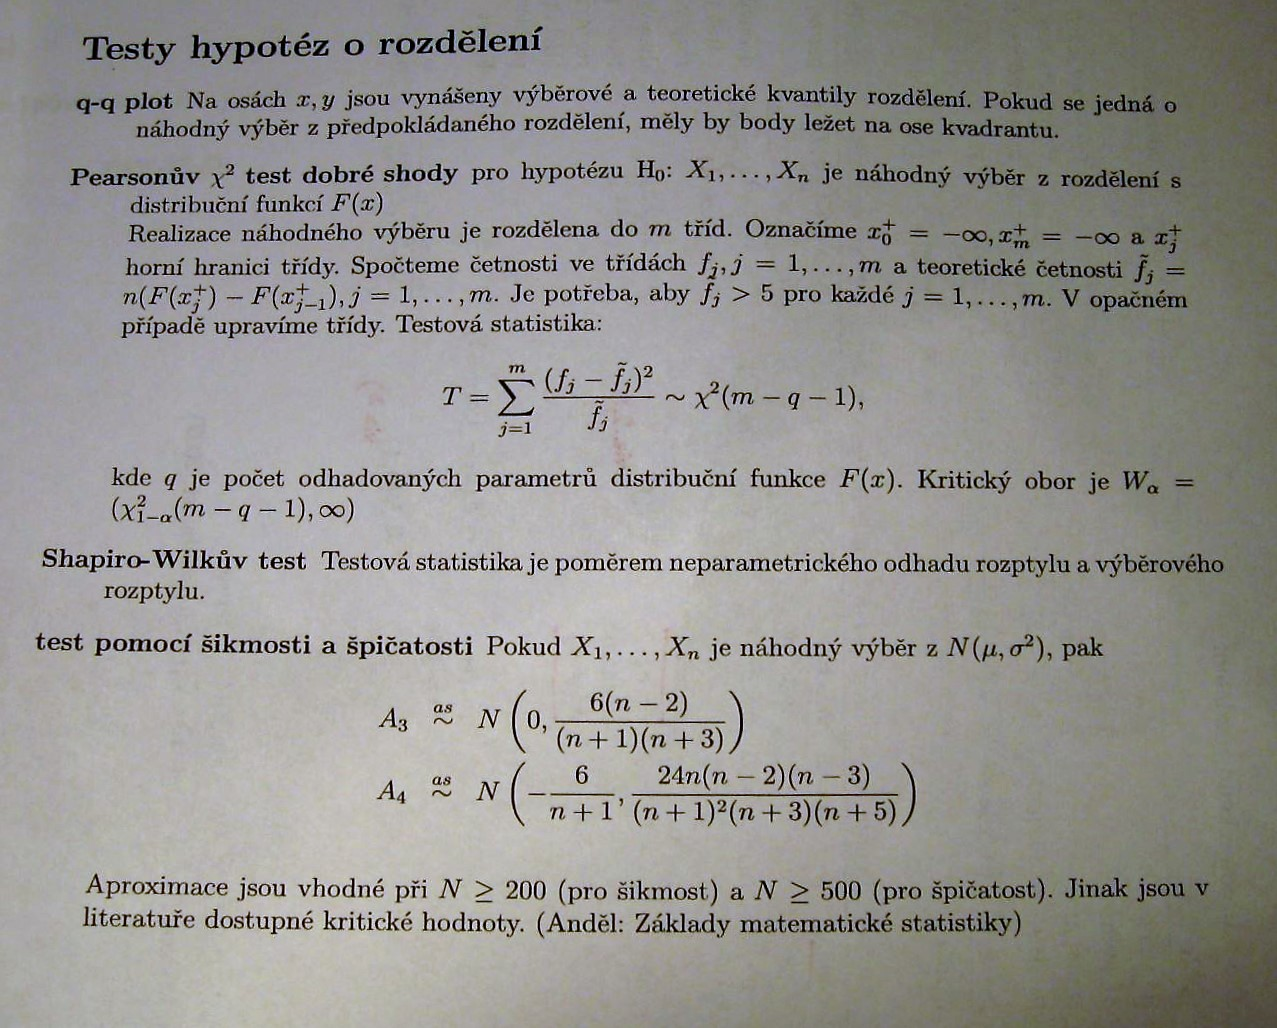
\includegraphics[scale=1]{Obrazky/stat4.png}
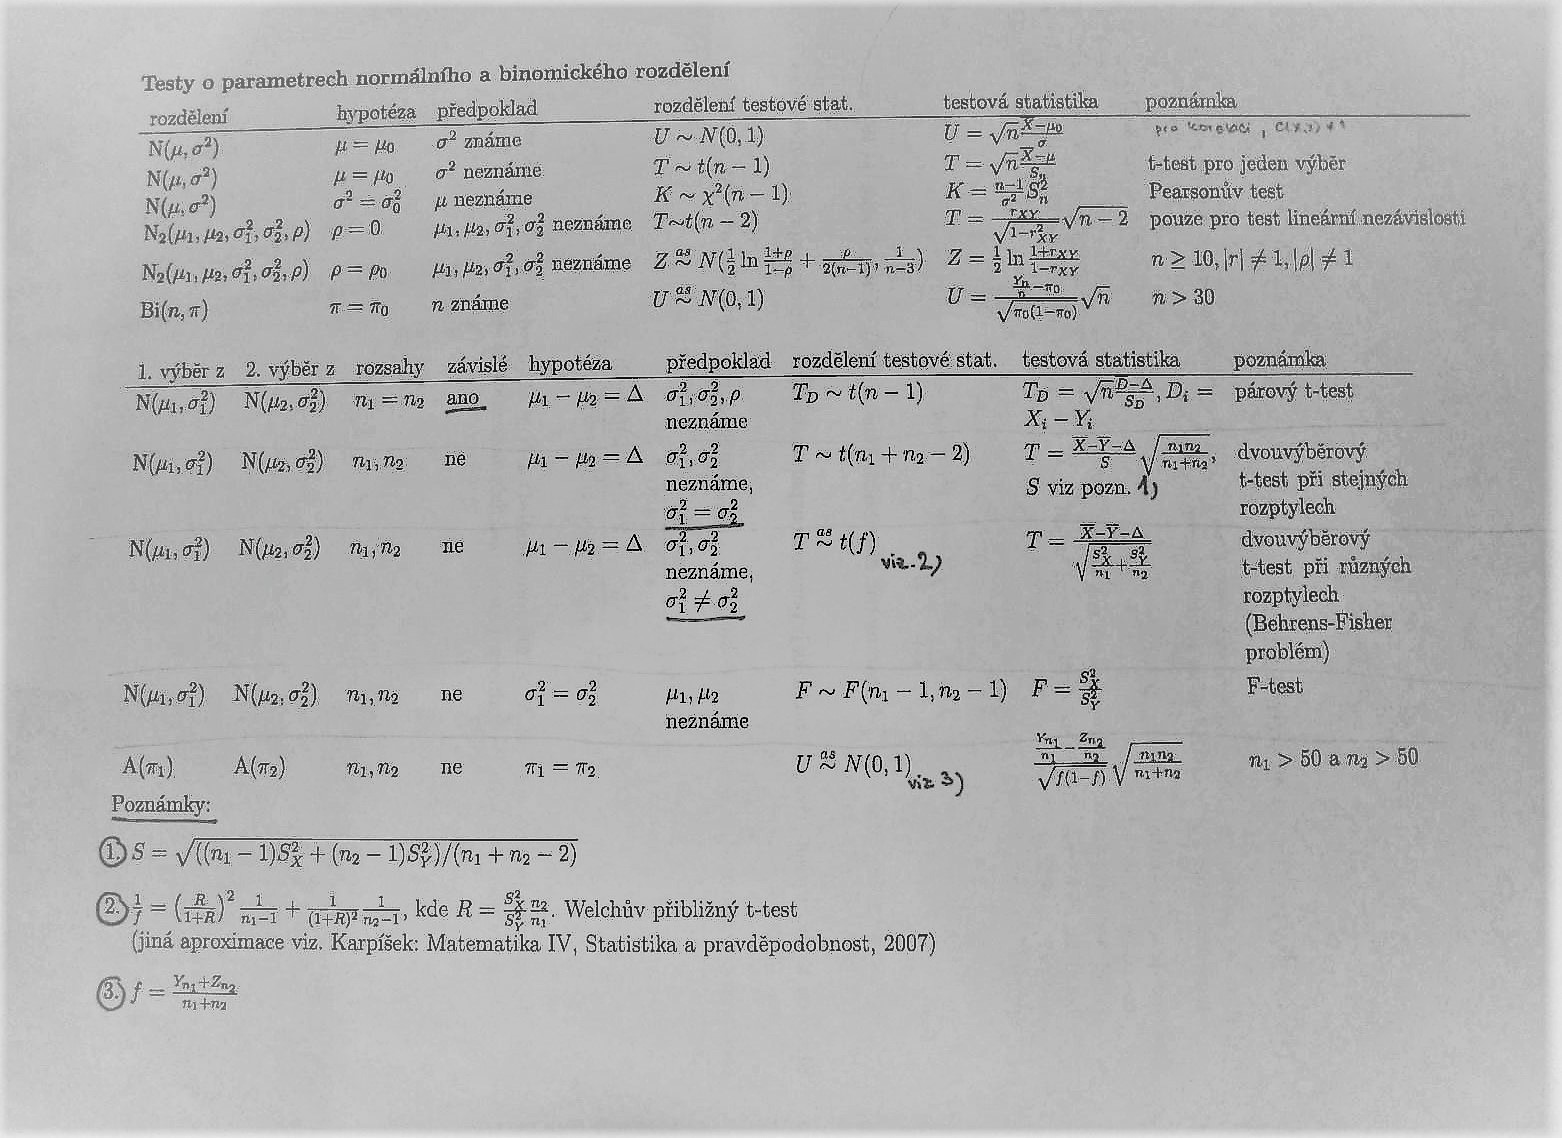
\includegraphics[scale=1]{Obrazky/stat2.png}
\end{figure}

\newpage
\section{Regresní analýza}



lineární regresní model, metoda nejmenších čtverců, bodové a intervalové odhady parametrů, testy hypotéz o regresních koeficientech, regresní diagnostika, nelineární model, korelační analýza.

Toto téma je zpracované na MATEMATIKA Online pro strojaře. Odkaz na stránky s PDF (musí se okopírovat odkaz do nového okna) mathonline.fme.vutbr.cz/Regresni-analyza/sc-1159-sr-1-a-185/default.aspx

\subsection{Lineární regresní model}
Hledání a zkoumání závislosti proměnných, které získáme jako reálná data z experimentu.

\begin{itemize}
    \item $Y, X_1,..., X_k$ náhodné veličiny na $(\Omega, \pmb{\mathcal{A}}, P)$
    \item $X_1,..., X_k$ jsou nezávislé proměnné
    \item $Y$ je závislá proměnná
    \item $\hat{Y} = \beta_1 X_1 + ... + \beta_k X_k$, kde $\beta_1, ..., \beta_k$ jsou neznámé parametry
    \item $E (Y - \hat{Y})^{2}$ je střední kvadratická chyba predikce
    \item Hledáme parametry $\beta_0$ a $\pmb{\beta}$ tak, aby $E (Y - \hat{Y})^{2}$ byla minimální 
    \item vezmeme-li $X_1 = x_1, ..., X_k = x_k$ pak    DOPLNIT, kde $e$ je náhodná chyba
    \item $Y, x_1,..., x_k$ pozorujeme (měříme) $n$ krát
    \item $Y_i, x_{i1},..., x_{ik}$ $i$-té pozorování $Y, x_1,..., x_k$ pro $i=1,2,...,n$
    \item Můžeme tedy napsat soustavu rovnic \begin{align*}
Y_1 &= \beta_1 x_{11} + ... + \beta_k x_{1k} + e_1 \\
    Y_2 &= \beta_1 x_{21} + ... + \beta_k x_{2k} + e_2 \\
    \vdots \\
    Y_n &= \beta_1 x_{n1} + ... + \beta_k x_{nk} + e_n    
\end{align*} 
    Pak $$\mathbf{Y} = \mathbf{X} \pmb{\beta} + \mathbf{e}$$ 
\end{itemize}

\begin{predpoklady}
\itemize
    \item $E\mathbf{e}=\mathbf{0}$
    \item var$\mathbf{e}=\sigma^2 \mathbf{I},$ kde $\sigma^2 > 0$ je neznámý parametr 
\end{predpoklady}

\begin{definition}
Model 
\begin{align*}
\mathbf{Y} &= \mathbf{X} \pmb{\beta} + \mathbf{e} \\
E \mathbf{Y} &= \mathbf{X} \pmb{\beta} \\
\mathrm{var} \, \mathbf{Y} = \mathrm{var} \, \mathbf{e} &= \sigma^{2} \mathbf{I} 
\end{align*}
nazýváme \textit{lineární regresní model} a značíme LRM($\mathbf{Y}$, $\mathbf{X} \pmb{\beta}$, $\sigma^2 \mathbf{I}$). Matici $\mathbf{X}$ nazýváme \textit{matice plánu}. Při h$(\mathbf{X})=k$ mluvíme o modelu plné hodnosti a při h$(\mathbf{X})<k$ mluvíme o modelu neúplné hodnosti.
\end{definition}

\begin{definition}
Řekneme, že náhodný vektor $\mathbf{T}$ je lineárním odhadem vektorové parametrické funkce $\pmb{\gamma} = \mathbf{C} \pmb{\beta}$, kde $\mathbf{C}$ je matice reálných čísel typu $m \times k$, jestliže $\mathbf{T} = \mathbf{BY}$, kde $\mathbf{B}$ je matice reálných čísel typu $m \times n$.
\end{definition}

Parametry $\beta_1, ..., \beta_k$ se odhadují \textit{metodou nejmenších čtverců}.

%%%%%%%%%%%%%%%%%%%%%%%%%%%%%%%%%%%%%%%%%%%%%%%%%%%%%%%%%%%%%%%%%%%%%%%%%%%%%%%%%%%%%%%%%%%%%%%%%%%%%%%%%%%%%%%%%%%%%%%%%%%%%%%%%%%%%%%%%%%%%%%%%%%%%%%%%%%%%%%%%%%%%%%%%%%%%%%%%%%%%%%%%%%%%%%%%%%%%%%
\subsection{Metoda nejmenších čtverců} 
\begin{definition}
Řekneme, že $\pmb{\hat{\beta}}$ je odhadem $\pmb{\beta}$ metodou nejmenších čtverců v LRM($\mathbf{Y}$, $\mathbf{X} \pmb{\beta}$, $\sigma^2 \mathbf{I}$), jestliže 
$$ S_{e}^{2} \left( \pmb{\hat{\beta}} \right) \leq S_{e}^{2} \left( \pmb{\beta} \right), \pmb{\beta} \in R ^ n ,$$ kde $ S_{e}^{2} \left( \pmb{\beta} \right) = \sum^{n}_{i=1} e_{i}^{2} = \sum^{n}_{i=1} \left( Y_i - \sum^{k}_{j=1} x_{ij} \beta_j \right) ^2 = \mathbf{e}^T \mathbf{e} = \left( \mathbf{Y} - \mathbf{X} \pmb{\beta} \right) ^T \left( \mathbf{Y} - \mathbf{X} \pmb{\beta} \right) $ 
\end{definition}

\begin{theorem}
Odhadem parametru $\pmb{\beta}$ metodou nejmenších čtverců v LRM($\mathbf{Y}$, $\mathbf{X} \pmb{\beta}$, $\sigma^2 \mathbf{I}$) je dán vztahem $$\pmb{\hat{\beta}} = \left( \mathbf{X}^T \mathbf{X} \right) ^{-1} \mathbf{X}^T \mathbf{Y}.$$
\end{theorem}

\begin{notes}$$
\hat{Y} = \mathbf{\beta_0} + \pmb{\beta}^T \mathbf{X} = E Y - \pmb{\beta}^T E \mathbf{X} + \pmb{\beta}^T \mathbf{X} = E Y - C\left( Y, \mathbf{X} \right) \left( D \mathbf{X} \right) ^ {-1} \left( \mathbf{X} - E \mathbf{X} \right)$$
je \textit{lineární regresní funkce}. 

$$min E (Y - \hat{Y})^{2} = DY - C\left( Y, \mathbf{X} \right) \left( D \mathbf{X} \right) ^ {-1} C \left( \mathbf{X}, Y \right) = \sigma^{2}_{Y \cdot \mathbf{X} }$$ je reziduální rozptyl.
\\ ($D \mathbf{X}$ je jiné značení variační matici var$\mathbf{X}$)
\end{notes}

%%%%%%%%%%%%%%%%%%%%%%%%%%%%%%%%%%%%%%%%%%%%%%%%%%%%%%%%%%%%%%%%%%%%%%%%%%%%%%%%%%%%%%%%%%%%%%%%%%%%%%%%%%%%%%%%%%%%%%%%%%%%%%%%%%%%%%%%%%%%%%%%%%%%%%%%%%%%%%%%%%%%%%%%%%%%%%%%%%%%%%%%%%%%%%%%%%%%%%%%%
\subsection{Bodové a intervalové odhady parametrů}
\begin{theorem}
Nechť vektor \pmb{Y} v LRM má $N_n\left(\pmb{X} \pmb{\beta}, \sigma^2 \pmb{I} \right).$ Pak statistika $$T = \frac{\pmb{c}^T \hat{\pmb{\beta}} - \pmb{c}^T \pmb{\beta}}{s \sqrt{\pmb{c}^T \left(\pmb{X}^T \pmb{X} \right)^{-1} \pmb{c}} } \sim t \left(n-k \right),$$ pro libovolné $0 \neq \pmb{c} \in \pmb{R}^k.$ 
\end{theorem}

\begin{notes}
Interval spolehlivosti $\beta_j, j \in \{1, \ldots , k \}$ $$P\left(-t_{1-\frac{\alpha}{2}} \left(n-k \right) \leq T_j \leq t_{1-\frac{\alpha}{2}} \left(n-k \right) \right) = 1- \alpha.$$ 
\end{notes}
%%%%%%%%%%%%%%%%%%%%%%%%%%%%%%%%%%%%%%%%%%%%%%%%%%%%%%%%%%%%%%%%%%%%%%%%%%%%%%%%%%%%%%%%%%%%%%%%%%%%%%%%%%%%%%%%%%%%%%%%%%%%%%%%%%%%%%%%%%%%%%%%%%%%%%%%%%%%%%%%%%%%%%%%%%%%%%%%%%%%%%%%%%%%%%%%%%%%%%%%%
\subsection{Testy hypotéz o regresních koeficientech}
Test hypotézy $H_0 : \gamma = \pmb{c}^T \pmb{\beta} = \gamma_0$ proti $H_1: \gamma \neq \gamma_0$. $H_0$ zamítáme na hladině významnosti $\alpha$ pokud $\gamma_0$ neleží v intervalu spolehlivosti. 
$$\left(\pmb{c}^T \hat{\pmb{\beta}} - t_{1-\frac{\alpha}{2}} \left(n-k \right)  s \sqrt{\pmb{c}^T \left(\pmb{X}^T \pmb{X} \right)^{-1} \pmb{c}},\pmb{c}^T \hat{\pmb{\beta}} + t_{1-\frac{\alpha}{2}} \left(n-k \right) s \sqrt{\pmb{c}^T \left(\pmb{X}^T \pmb{X} \right)^{-1} \pmb{c}} \right) $$

%%%%%%%%%%%%%%%%%%%%%%%%%%%%%%%%%%%%%%%%%%%%%%%%%%%%%%%%%%%%%%%%%%%%%%%%%%%%%%%%%%%%%%%%%%%%%%%%%%%%%%%%%%%%%%%%%%%%%%%%%%%%%%%%%%%%%%%%%%%%%%%%%%%%%%%%%%%%%%%%%%%%%%%%%%%%%%%%%%%%%%%%%%%%%%%%%%%%%%%%%
\subsection{Regresní diagnostika}
%%%%%%%%%%%%%%%%%%%%%%%%%%%%%%%%%
\subsubsection{Ověření stability}
$\hat{\mathbf{e}} \sim N(\mathbf{0}, \sigma^{2} \mathbf{M})$

\begin{itemize}
    \item složky $\mathbf{e}$ nemusí mít stejný rozptyl $\Rightarrow$ standardizované $v_i = \frac{\hat{e}_t}{s \sqrt{m_{ii}}}$
    \item v grafu $(i, v_i)$ hledáme trend
    \item v grafu $(x_i, v_i)$ hledáme \begin{itemize}
    \item velké hodnoty
    \item trend
    \item oblasti s různým rozptylem - Barlettův test
    \end{itemize}
\end{itemize}
%%%%%%%%%%%%%%%%%%%%%%%%%%%%%%%%%%%%%%
\subsubsection{Ověření nezávislosti}
Složky $\hat{e}_i$ mohou být závislé. 
\textit{Durbin-Watson test} nezávislosti (u posloupnosti) 
$$d = \frac{\sum_{i=1}^{n-1} \left( e_{i+1}+e_i\right) ^ 2}{\sum_{i=1}^{n} e_i ^ 2} \in \langle 0, \, 4 \rangle $$ Kritické hodnoty $d_L (\alpha)$, $d_U (\alpha)$ lze nalézt v tabulkách (pokud matice plánu má sloupec jedniček): \\
$d < d_L (\alpha)$ zamítáme nazávislost \\
$d_L (\alpha) < d < d_U (\alpha)$ test je neprůkazný \\
$d_U (\alpha) < d$ nezamítáme nezávislost \\
Jinak jsou hodnoty $\hat{e}$ závislé na $\mathbf{X}$. 

%%%%%%%%%%%%%%%%%%%%%%%%%%%%%%%%%
\subsubsection{Ověření normality}
\begin{itemize}
    \item Q-Q plot: empirický vs. teoretický kvantil 
    \item P-P plot
    \item test normality: Pearson $\chi ^2$, Shapiro-Wilks, Anderson-Darling (citlivý na zaokrouhlování) 
\end{itemize}

%%%%%%%%%%%%%%%%%%%%%%%%%%%%%%%%%%%%%%
\subsubsection{Koeficient determinace}
\begin{itemize}
    \item porovnávání $S_{e}^{2}$ v minimálním modelu (označení $SS_T$) s $S_{e}^{2}$ ve odhadovaném modelu 
    \item $S_{e}^{2} = \sum_{i=1}^{n} \left( Y_i - \hat{Y} \right)^2$
    \item $SS_{T} = \sum_{i=1}^{n} \left( Y_i - \bar{Y} \right)^2$
    \item Koeficient determinace: $R^2 = 1 -\frac{S_{e}^{2}}{SS_{T}}$ určuje procento variabylity $\mathbf{Y}$ vysvětlené modelem (čím blíže k 1, tak je model "lepší" na popsání dat, $R^2$ leží od 0 po 1 včetně)
    \item Korigovaný koeficient determinace:  $R_{adj}^{2} = 1 -\frac{n-1}{n-k} \frac{S_{e}^{2}}{SS_{T}}$
\end{itemize}

%%%%%%%%%%%%%%%%%%%%%%%%%%%%%%%%%%%%%
\subsubsection{Leverage = vlivný bod}
\begin{itemize}
    \item změna (vynechání) hodnoty $y_i$, která způsobý značnou změnu $\hat{y}_i$
    \item $\hat{\mathbf{Y}} = \mathbf{X} \left( \mathbf{X}^T \mathbf{X} \right) \mathbf{X} ^T \mathbf{Y}$
    \item pokud je složka vektoru $m_i$, kde $\mathbf{M} = \mathbf{X} \left( \mathbf{X}^T \mathbf{X} \right) \mathbf{X} ^T$, malá $\implies$ $y_i$ není vlivný bod 
\end{itemize}

%%%%%%%%%%%%%%%%%%%%%%%%%%%%%%%%%%%%%%%%%%%%%%%%%%%%%%%%%%%%%%%%%%%%%%%%%%%%%%%%%%%%%%%%%%%%%%%%%%%%%%%%%%%%%%%%%%%%%%%%%%%%%%%%%%%%%%%%%%%%%%%%%%%%%%%%%%%%%%%%%%%%%%%%%%%%%%%%%%%%%%%%%%%%%%%%%%%%%%%%%%%%%%%%%%%%%%%%%%%%
\subsection{Nelineární regresní modely}
\begin{itemize}
\item Linearizovatelná regrese $$Y_i = \beta_0 \exp \{\beta_i x_i + e_i \},\, i=1,\ldots, n$$ $\beta_0, \beta_1$ jsou neznámé parametry a $e_i$ jsou chyby.
\item Bilineární regrese $$Y_i = \beta_1 \exp \{\beta_2 x_i \} + \beta_3 \exp \{\beta_4 z_i \}+ e_i,\,i=1,\ldots, n,$$ $\beta_1, \ldots, \beta_4$ jsou neznámé parametry a $e_i$ jsou chyby. Předpokládáme, že známe počáteční odhady parametrů $\hat{\beta_{10}}$ a $\hat{\beta_{20}}$. Parametry $\beta_i$ určujeme iteračně.
\item Obecný případ $$Y_i = f\left(x_i,\pmb{\beta} \right) + e_i,\,i=1,\ldots, n, $$ $E e_i = 0, D e_i = \sigma^2, \pmb{\beta} \in \mathtt{R}^k.$ Odhad $\pmb{\beta}$ určíme minimalizací metodou nejmenších čtverců $ s^2 \left(\pmb{\beta} \right) = \sum_{i=1}^{n} \left( Y_i - f \left(x_i,\pmb{\beta} \right) \right)^2.$
\end{itemize}

%%%%%%%%%%%%%%%%%%%%%%%%%%%%%%%%%%%%%%%%%%%%%%%%%%%%%%%%%%%%%%%%%%%%%%%%%%%%%%%%%%%%%%%%%%%%%%%%%%%%%%%%%%%%%%%%%%%%%%%%%%%%%%%%%%%%%%%%%%%%%%%%%%%%%%%%%%%%%%%%%%%%%%%%%%%%%%%%%%%%%%%%%%%%%%%%%%%%%%%%%%%%%%%%%%%%%%%%%%%%
\subsection{Korelační analýza}
\begin{definition}
\textit{Koeficientem mnohonásobné korelace} mezi náhodnou veličinou $Y$ a náhodným vektorem $\pmb{X} = \left(X_1,\ldots, X_k \right)^T$ rozumíme číslo $\rho_{Y,\pmb{X}} = R \left( Y, \hat{Y} \right),$ kde $\hat{Y} = E Y + C \left(Y, \pmb{X} \right) \left(\pmb{X}\right)^{-1}\left(\pmb{X}- E \pmb{X} \right)$. Definuje míru lineární stochastické závislosti mezi náhodnou veličinou $Y$ a vhodnou lineární kombinací složek $X_1$, $X_2$, \ldots, $X_n$ náhodného vektoru $\mathbf{X}$.
\end{definition}

\begin{theorem}
Pro koeficient mnohonásobné korelace platí
\begin{itemize}
\item $\rho_{Y, \mathbf{X}} \geq 0$
\item $\rho_{Y, \mathbf{X}}^2 = \frac{\bm{\hat{\beta}}^T D \mathbf{X} \bm{\hat{\beta}}}{D Y}$
\item $\rho_{Y, \mathbf{X}}^2 = R(Y, \mathbf{X}) \cdot R(\mathbf{X})^{-1} \cdot R(\mathbf{X}, Y)$
\item $\rho_{Y, \mathbf{X}}^2 = 1 - \frac{\sigma_{Y, \mathbf{X}}^2}{D Y}$
\end{itemize}
\end{theorem}

\begin{definition}
Mejme predikce
\begin{align*}
\hat{Y} &= \hat{\beta_0} + \bm{\hat{\beta}}^T \mathbf{X}, & \text{ kde } \bm{\hat{\beta}} =  C(Y, \mathbf{X}) D \mathbf{X}^{-1}\\
\hat{Z} &= \hat{\gamma_0} + \bm{\hat{\gamma}}^T \mathbf{X} & \text{ kde } \bm{\hat{\gamma}} =  C(Z, \mathbf{X}) D \mathbf{X}^{-1}.
\end{align*}
Korelaci $R(Y - \hat{Y}, Z - \hat{Z})$ nazyvame parialni korelacni koeficient nahodnych velicin $Y$ a $Z$ pri danem vektoru $\mathbf{X}$ a znacime ji $\rho_{Y, Z \cdot \mathbf{X}}$. Definuje míru lineární závislosti mezi náhodnými veličinami Y a Z při zkonstantnění složek vektoru X (při zrušení vlivu změny složek vektoru X ).
\end{definition} 

\begin{theorem}
Pro parcialni korelacni koeficient plati
\begin{equation*}
\rho_{Y, Z \cdot \mathbf{X}} = \frac{R(Y, Z) - R(Y, \mathbf{X}) (R(\mathbf{X}))^{-1} R(\mathbf{X}, Z)}{\sqrt{(1 - \rho_{Y, \mathbf{X}}^2)(1 - \rho_{Z, \mathbf{X}}^2)}}
\end{equation*}
\end{theorem}

\begin{definition}
Výběrový korelační koeficient je dan vzrocem
$$r _{\pmb{X} \pmb{Y}} = \frac{S_{\pmb{X} \pmb{Y}}}{S_{\mathbf{X}} S_{\mathbf{Y}}},$$ kde $S_{\mathbf{X}}, S_{\mathbf{Y}} \neq 0$, $s_{\pmb{X}}^2 = \frac{1}{n-1} \sum_{i=1}^{n} \left(x_i - \bar{X} \right)^2,$ $\bar{X} = \frac{1}{n} \sum_{i=1}^{n} x_i$ a $s_{\pmb{X},\pmb{Y}} = \frac{1}{n-1} \sum_{i=1}^{n} \left(x_i - \bar{X} \right)\left(y_i - \bar{Y} \right)$.
\end{definition}

\begin{theorem}
Necht $(X_1, Y_1)^T$, $\ldots$, $(X_N, Y_N)^T$ je nahodny vyber z dvojrozmerneho normalniho rozdeleni $N_2 (\mu_1, \mu_2, \sigma_1, \sigma_2, \rho)$, $n >2$. Potom za predpokladu $\rho = 0$ 
\begin{equation*}
T = \frac{r_{X Y}}{\sqrt{1 - r_{XY}^2}} \sqrt{n - 2} \sim t(n - 2).
\end{equation*}
\end{theorem}

\begin{definition}
Vyberovy koeficient mnohonasobne korelace je
\begin{align*}
r_{Y, \mathbf{X}} &= \sqrt{R_{Y \mathbf{X}} \cdot R_{\mathbf{X} \mathbf{X}}^{-1} \cdot R_{\mathbf{X} Y}},\\
\text{specialne pro } \mathbf{X}=(X,Z): r_{Y, XZ} &= \sqrt{\frac{r_{XY}^2 - 2 r_{XZ} r_{XY} r_{YZ} + r_{YZ}^2}{1 - r_{XZ}}} \\
\text{a pro } H_0: \rho_{Y, \mathbf{X}} = 0: Z &= \frac{n - p - 1}{p} \frac{r_{Y, \mathbf{X}}^2}{1 - r_{Y, \mathbf{X}}^2} \sim F(p, n - p - 1).
\end{align*}

Vyberovy koeficient parcialni korelace je
\begin{align*}
r_{Y,Z \cdot \mathbf{X}} &= \frac{r_{Y,Z} - R_{Y, \mathbf{X}} R_{\mathbf{X}, \mathbf{X}}^{-1} R_{\mathbf{X}, Z}}{\sqrt{(1 - R_{Y, \mathbf{X}} R_{\mathbf{X}, \mathbf{X}}^{-1} R_{\mathbf{X}, Y}) (1 - R_{YZ, \mathbf{X}} R_{\mathbf{X}, \mathbf{X}}^{-1} R_{\mathbf{X}, Z})}}\\
\text{specialne pro } \mathbf{X} = X: r_{Y, Z \cdot \mathbf{X}} &= \frac{r_{YZ} - r_{YX} r_{ZX}}{\sqrt{(1 - r_{YX}^2) (1 - r_{ZX}^2)}} \\
\text{a pro } H_0: \rho_{Y,Z \cdot \mathbf{X}} = 0: T &= \frac{r_{Y,Z \cdot \mathbf{X}}}{\sqrt{1 - r_{Y,Z \cdot \mathbf{X}}^2}} \sqrt{n - p -2} \sim t(n - p - 2).
\end{align*}
\end{definition}

%%%%%%%%%%%%%%%%%%%%%%%%%%%%%%%%%%%%%%%%%%%%%%%%%%%%%%%%%%%%%%%%%%%%%%%%%%%%%%%%%%%%%%%%%%%%%%%%%%%%%%%%%%%%%%%%%%%%%%%%%%%%%%%%%%%%%%%%%%%%%%%%%%%%%%%%%%%%%%%%%%%%%%%%%%%%%%%%%%%%%%%%%%%%%%%%%%%%%%%%%%%%%%%%%%%%%%%%%%%%
%\itemize{Zdroje:}
%    \item Anděl, J., Základy matematické statistiky, Praha 2013
%    \item Hübnerová, Z., Studijní materiály pro SP2, Brno 2016


\section{Statistická analýza}
testy hypotéz o parametrech normálního rozdělení (t-test a F-test), analýza rozptylu, neparametrické testy, testy dobré shody, analýza 
kategoriálních dat.

\subsection{Testy hypotéz o parametrech normálního rozdělení (t-test a F-test)}
2. kapitola 
\url{http://mathonline.fme.vutbr.cz/Testovani-statistickych-hypotez/sc-1158-sr-1-a-154/default.aspx}

\subsection{Analýza rozptylu}

Analysis of variance = ANOVA

Dělali jsme pouze jednoduché třídění/jednoduchá ANOVA

Máme nezávislé výběry z rozdělení $N\left(\mu_1,\sigma^2\right),\ldots,\,N\left(\mu_I,\sigma^2\right)$ a testujeme hypotézu $H_0:\mu_1=\ldots=\mu_I$ přičemž parametr $\sigma^2$ není znám. U ANOVA je předpoklad rovnosti rozptylů náhodných výběrů, které jsou navzájem nezávislé a testujeme s2hodnost středních hodnot. 

Str. 47 a 48
\url{https://www.dropbox.com/home/SP2\%20-\%20Pravd\%C4\%9Bpodobnost\%20a\%20statistika\%20II?preview=reg.pdf}

Anděl od strany 210 do 215. 

\subsection{Neparametrické testy}
\url{https://www.dropbox.com/home/SP3\%20-\%20Pravd\%C4\%9Bpodobnost\%20a\%20statistika\%20III/Zuz\%C4\%8Diny\%20origin\%C3\%A1ln\%C3\%AD\%20pdf?preview=08_Neparametricketesty.pdf}
\url{https://www.dropbox.com/home/SP2\%20-\%20Pravd\%C4\%9Bpodobnost\%20a\%20statistika\%20II?preview=u15.pdf}

Na základě hodnot náhodného výběru činíme rozhodnutí o platnosti hypotézy o hodnotách parametrů rozdělení nebo o jeho vlastnostech. Rozeznáváme dva základní typy testů:

\textbf{Parametrické testy} jsou testy o hodnotách parametrů rozdělení, ze kterého je proveden náhodný výběr.

\textbf{Neparametrické testy} jsou testy o typu rozdělení, shodě rozdělení, symetrii rozdělení.

Testování provádíme na základě funkce náhodného výběru, statistiky, jejíž rozdělení je známé a rozhodnutí činíme na základě hodnot této statistiky.

\textbf{Příklady neparametrických testů:} \begin{itemize}
\item Znaménkový test: $X_1,\ldots,X_n$ je náhodný výběr ze spojitého rozdělení s jediným mediánem $\tilde{x}$. $$P\left(X_i < \tilde{x} \right) = P\left(X_i > \tilde{x} \right) = 0,5,\, i=1,\ldots, n$$ $H_0: \tilde{x} = x_0$ proti $H_1: \tilde{x} \neq x_0$. Má malou sílu, ale je vhodný pro sešikmená data. 
\item Jednovýběrový Wilcoxonův test: $X_1,\ldots,X_n$ je náhodný výběr ze spojitého rozdělení s hustotou $f$, která je symetrická kolem $a$ a kladná v jeho okolí $f\left(a-x\right)=f\left(a+x\right)$. Proto $\tilde{x}=a$, existuje $EX_i = a$. $H_0: \tilde{x} = x_0$ proti $H_1: \tilde{x} \neq x_0$. 
\item Dvouvýběrový Wilcoxonův test: $X_1,\ldots,X_m$ je náhodný výběr ze spojitého rozdělení s distribuční funkcí $F$ a $Y_1,\ldots,Y_n$ je náhodný výběr ze spojitého rozdělení s distribuční funkcí $G$. $H_0: F = G$ proti $H_1: F \neq G$. Test je citlivý zvláště na posunutí.
\item Kolmogorovův-Smirnovův test: využívá empirická distribuční funkce. 
\item Kruskalův-Walisův test: zobecnění 2 výběrového Wilcoxna - jednoduchá ANOVA. Citlivý na posunutí.
\item Spearmanův korelační koeficient
\end{itemize}
\subsection{Testy dobré shody}
\url{https://www.dropbox.com/home/SP2\%20-\%20Pravd\%C4\%9Bpodobnost\%20a\%20statistika\%20II?preview=materialyS2P.pdf}
8. kapitola

\subsection{Analýza kategoriálních dat}
\textbf{Pearsonův test nezávislosti a homogenity}

Nechť $(X,Y)$ je náhodný vektor s konečným sdruženým rozdělením pravděpodobnosti. Vektor $X$ nabývá hodnot $i = 1, \ldots, r, r \geq 2$ a $Y$ nabývá hodnot $j = 1, \ldots, c, c \geq 2$. Předpokládejme, že rozsah výběru $n \geq 4$, $n_{ij}$ je počet případů, kdy se vyskytla dvojice $(i, j)$, matice absolutních četností $[n_{ij}]_{i,j}$ má multinomické rozdělení s parametrem $n$ a pravděpodobnostmi $p_{ij}$. Pozorované hodnoty zapíšeme do kontingenční tabulky, kde
\begin{align*}
& \text{marginální četnosti }
\begin{cases}
n_{i \boldsymbol{\cdot}} = \sum_j n_{ij}\\
n_{\boldsymbol{\cdot} j} = \sum_i n_{ij}
\end{cases} \\
n =& \sum_i n_{i \boldsymbol{\cdot}} = \sum_j n_{\boldsymbol{\cdot} j} = \sum_i \sum_j n_{ij}.
\end{align*}

\begin{figure}[H]
\centering
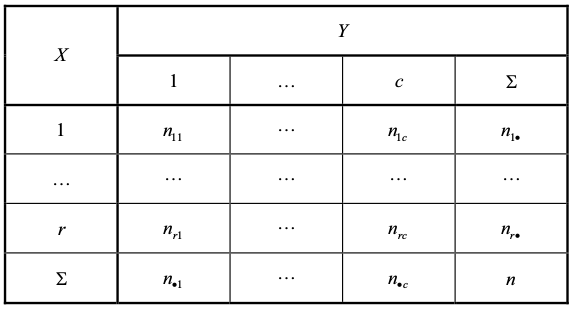
\includegraphics[width=0.8\textwidth]{Obrazky/kontingencni_tabulka.png}
\caption{Kontingenční tabulka}
\end{figure}

\textbf{Test nezávislosti $X$ a $Y$}

Je ekvivalentní testu $H_0: p_{ij} = p_{i \boldsymbol{\cdot}} p_{\boldsymbol{\cdot} j}, \forall (i,j)$, kde $p_{i \boldsymbol{\cdot}} = \sum_j p_{ij}, p_{\boldsymbol{\cdot} j} = \sum_i p_{ij}$ jsou marginální pravděpodobnosti složek $X$ a $Y$ náhodného vektoru $(X,Y)$. Hypotézu $H_0$ testujeme pomocí Pearsonova testového kritéria
\begin{equation*}
\chi^2 = \sum_{i = 1}^r \sum_{ j = 1}^c \frac{(n_{ij} - \frac{n_{i \boldsymbol{\cdot}} n_{\boldsymbol{\cdot} j}}{n})^2}{\frac{n_{i \boldsymbol{\cdot}} n_{\boldsymbol{\cdot} j}}{n}} = n \sum_{i = 1}^r \sum_{ j = 1}^c \frac{n_{ij}^2}{n_{i \boldsymbol{\cdot}} n_{\boldsymbol{\cdot} j}} - n.
\end{equation*}

Hypotézu $H_0$ nezamítáme na hladině významnosti $\alpha$, jestliže $\chi^2 \in \bar{W}_{\alpha} = \langle 0; \chi^2_{1 - \alpha} ((r - 1)(c - 1)) \rangle$. Tento test je asymptotický, obvykle požadujeme, aby pro dvojici $(i,j)$ bylo $\frac{n_{i \boldsymbol{\cdot}} n_{\boldsymbol{\cdot} j}}{n} > 5$.

%\itemize{\textbf{Zdroje:}}
%    \item Anděl, J., Základy matematické statistiky, Praha 2013
%    \item Hübnerová, Z., Studijní materiály pro SP3, Brno 2016

\textbf{Test homogenity}

Testujeme hypotézu, ze pozorované četnosti ve všech řádcích kontingenční tabulky mají multinomické rozdělení s parametry $n_{i \boldsymbol{\cdot}}$ a stejnými pravděpodobnostmi $q_j = p_{1j} = \ldots = p_{rj}$ pro $j = 1, \ldots, c$.

Jestliže $r = c = 2$, jde o tzv. čtyřpolní tabulku pro alternativní (dichotomické) statistické znaky $X$ a $Y$, např. odpovědi respondentů, "ano" nebo "ne".

%%%%%%%%%%%%%%%%%%%%%%%%%%%%%%%%%%%%%
\section{Digitální obraz}

\section{Stochastické procesy}

\section{Filtrace obrazu}

\section{Segmentace a rozpoznávání objektu}



\section{Statistika pro loosery 5.2}
\begin{notes}
Alternativní definice podle Zuzany
\end{notes}
\begin{definition}{(\textbf{Náhodná veličina})}
Nechť $( \Omega, \mathcal{A}) $ je jevové pole a $(\mathbb{R}, \mathcal{B})$ je měřitelný prostor ( tj. $\mathcal{B}$ je borelovská $\sigma$-algebra). Zobrazení $X:\Omega \rightarrow \mathbb{R}$ se nazývá \textit{náhodná veličina} vzhledem k $\mathcal{A}$ právě, když úplný vzor každé borelovské množiny je jev vzhledem k $\mathcal{A}$, tj.
\begin{equation*}
\forall B \in \mathcal{B}: X^{inv }(B):=\{\omega\in \Omega : X(\omega)\in B \}\in \mathcal{A}
\end{equation*}
\end{definition}

\begin{theorem}
Nechť $( \Omega, \mathcal{A}) $ je jevové pole a $(\mathbb{R}, \mathcal{B})$ je měřitelný prostor ( tj. $\mathcal{B}$ je borelovská $\sigma$-algebra). Zobrazení $X:\Omega \rightarrow \mathbb{R}$ se nazývá \textit{náhodná veličina} vzhledem k $\mathcal{A}$ právě, když 
\begin{equation}
\forall x \in \mathbb{R} : \{ \omega \in \Omega: X(\omega)< x\}\in \mathcal{A}
\end{equation}
\end{theorem}


\begin{table}[h]
\centering
\caption{My caption}
\label{my-label}
\begin{tabular}{lll}
jev &zkrácený zápis jevu  & pravděpodobnost  \\
\hline
$\omega:X(\omega)\in B$ &$X\in B$  &$\textbf{P}(X\in B)$  \\
$\omega:X(\omega)< x$ &$X < x$  &$\textbf{P}(X<x)$  \\
$\omega:X(\omega)=x $ &$X=x$  &$\textbf{P}(X=x)$  
\end{tabular}
\end{table}



\begin{definition}
Nechť $(\Omega,\mathcal{A},\textbf{P})$ je pravděpodobnostní prostor a nechť $X$ je náhodná veličina vzhledem k $\mathcal{A}$. Pravděpodobnost $\textbf{P}_x:\mathcal{B}\rightarrow \mathbb{R}, \textbf{P}_x(B)=\textbf{P}(X\in B), \forall B\in \mathcal{B}$ se nazývá rozdělení pravděpodobnosti náhodné veličiny $X$
\end{definition}



\begin{definition}
Nechť $(\Omega,\mathcal{A},\textbf{P})$ je pravděpodobnostní prostor a nechť $X$ je náhodná veličina vzhledem k $\mathcal{A}$. Pak funkci $F_X(x)=\textbf{P}(X<x)$ definovanou pro každé $x\in \mathbb{R}  $ nazýváme distribuční funkcí náhodné veličiny $X$.
\end{definition}

\begin{theorem}
Nechť $(\Omega,\mathcal{A},\textbf{P})$ je pravděpodobnostní prostor a nechť $F(x)$ je její distribuční funkce. pak platí
\begin{enumerate}
\item $0\leq F(x)\leq 1\forall x \in \mathbb{R}$
\item F(x) je neklesající funkce
\item F(x) je zleva spojitá
\item $\lim_{x\rightarrow \infty}F(x)=1$ a  $\lim_{x\rightarrow -\infty}F(x)=0$
\item Pro libovolné $x_1,x_2 \in \mathbb{R}, x_1<x_2$ platí $\textbf{P}(x_1\leq X<x_2)=F(x_2)-F(x_1)$
\item $\forall a \in \mathbb{R}$ platí $\textbf{P}(X=a)=\lim_{x\rightarrow a^+} F(x)-F(x)$
\item $F(x)$ má nejvýše spočetně mnoho bodů nespojitosti
\item $\textbf{P}(a\leq X)=1-F(a) \forall a \in \mathbb{R}$
\item $P(X\leq a) = \lim_{x\rightarrow a^+} F(x) , \forall a \in \mathbb{R}$
\end{enumerate}
\end{theorem}

\begin{notes}
Z $(6)$ plyne, že distribuční funkce je v bodě $x$ spojitá $\Leftrightarrow \textbf{P}(X=x)=0$ 
\end{notes}


\begin{notes}
Mezi $\textbf{P}_X$ a $F$ je vzájemně jednoznačný vztah. řekneme, že distribuční funkce určuje rozdělení pravděpodobnosti náhodné veličiny $X$. Lebesgue-Stieltjes integrál: $\textbf{P}_X(B)=\int_B \mathrm{d}F(x)$
\end{notes}

\begin{theorem}
Má-li funkce $F(x):\mathbb{R}\rightarrow \mathbb{R} vlastnosti (2),(3) $ a $(4)$, pak existuje pravděpodobnostní prostor $\Omega,\mathcal{A},\textbf{P})$ a na něm definovaná náhodná veličina $X$ tak, že $F(x)$ je její distribuční funkcí.
\end{theorem}



\subsection{Diskrétní a spojité náhodné veličiny}
\begin{definition}
Nechť $(\Omega,\mathcal{A},\textbf{P})$ je pravděpodobnostní prostor.  Řekneme, že náhodná veličina $X$ je diskrétní (vzhledem k $P$) právě tehdy, když existuje neprázdná nejvýše spočetná množina $M \subset \mathbb{R}$ taková, že $\textbf{P}_X(M)=1$. Množina $M$ se nazývá obor hodnot a funkce \begin{equation}
p(x)=\textbf{P}(X=x),x\in \mathbb{R}
\end{equation}
se nazývá pravděpodobnostní funkcí diskrétní náhodné veličiny $X$.
\end{definition}

\begin{theorem}
Nechť $X$ je diskrétní náhodná veličina, která má obor hodnot $M$, pravděpodobnostní funkci $p$ a distribuční funkci $F(x)$. pak
\begin{enumerate}
\item $\forall x \in \mathbb{R}: p(x)\geq 0$ (nezápornost)
\item $\sum_{x\in M} p(x) =1$ (normovanost)
\item $F(x)=\sum_{y\in M \cap (-\infty,x\rangle } p(y) $ pro každé $x \in \mathbb{R}$
\item $P(X\in B)=\sum_{y\in M \cap B } p(y) $ pro každé $B \in \mathcal{B}$
\item $p(x) \leq 1$
\item $p(x)= \lim_{t\rightarrow x^+ }F(t)-F(x)$

\end{enumerate}
\end{theorem}

\begin{notes}
Distribuční funkce diskrétní náhodné veličiny má schodovitý průběh a určuje pravděpodobnostní funkci jednoznačně (viz $(6)$).
\end{notes}

\begin{theorem}
Nechť reálná funkce $p(x)$ má vlastnosti $(1),(2)$, pak existuje pravděpodobnostní prostor a na něm definovaná diskrétní náhodná veličina $X$ taková, že $p(x)$ je její pravděpodobnostní funkce.
\end{theorem}


\begin{definition}
Nechť $(\Omega,\mathcal{A},\textbf{P})$ je pravděpodobnostní prostor. Řekneme, že náhodná veličina $X$ s distribuční funkcí $F(x)$ je \textit{je spojitá} (vzhledem k $\textbf{P}$) právě tehdy, když existuje nezáporná po částech spojitá funkce $f(x)$, že pro $\forall x \in \mathbb{R}$ platí 
\begin{equation}
F(x)=\int_{-\infty}^x f(t)\, \mathrm{d} t.
\end{equation}
Funkce $f(x)$ se nazývá hustota náhodné veličiny $X$.
\end{definition}

\begin{notes}
Distribuční funkce spojité náhodné veličiny $X$ je všude spojitá, protože je funkcí horní meze integrálu.
\end{notes}

\begin{theorem}
Nechť $f(x)$ je hustota spojité náhodné veličiny $X$. Pak 
\begin{enumerate}
\item $f(x)\geq 0, \forall x \in \mathbb{R}$
\item $\int_{-\infty}^{\infty} f(x)\, \mathrm{d} x=1$
\item Pro libovolné ale pevně zvolené $x_0\in \mathbb{R}$ a $h>0 $ platí $P(x_0<X<x_0+h)=\int_{x_0}^{x_0+h}f(x)\, \mathrm{d}x$
\item Pro libovolné ale pevně dané $x_0\in \mathbb{R}$ platí $P(X=x_0)=0$
\item Ve všech bodech spojitosti funkce $f(x)$ platí$ \mathrm{d}F(x)/\mathrm{d}x$
\end{enumerate}
\end{theorem}

\begin{theorem}
Jestliže reálná funkce $f(x)$ má vlastnosti $(1),(2)$, pak existuje pravděpodobnostní prostor $(\Omega,\mathcal{A},\textbf{P})$ a na něm definovaná spojitá náhodná veličina $X$ tak, že $f(x)$ je její hustota.
\end{theorem}

\subsection{Rozdělení transformovaných náhodných veličin}
\begin{theorem}
Nechť $(\Omega, \mathcal{A})$ je jevová $\sigma$-algebra a $(\mathbb{R},\mathcal{B})$ je měřitelný prostor, $X:\Omega\rightarrow \mathbb{R}$ je náhodná veličina a $g:\mathbb{R}\rightarrow\mathbb{R}$ je borelovská funkce (tj. úplný vzor $\forall B \in \mathcal{B}$ je z $\mathbb{B}$). Pak složené zobrazení $Y:\Omega\rightarrow \mathbb{R}$ dané vzorcem $\forall \omega \in \Omega: Y(\omega)=g(X(\omega))$ je náhodná veličina (vzhledem k $\mathcal{A}$). zobrazení $Y$ nazýváme transformovaná náhodná veličina.
 \end{theorem}
 
 \begin{theorem}
 Nechť náhodná veličina $X$ má distribuční funkci $F_X$ a nechť $g$ je borelovská funkce. Pak transformovaná náhodná veličina $Y=g(X)$ má distribuční funkci $F_Y(y)=\int_{B_y}\mathrm{d}F(x)$, kde $B_y=\{x:h(x)<y) \}$
 \end{theorem}

\begin{notes}
Pro diskrétní veličinu $X$ s pravděpodobnostní funkcí $p$ lze $F_Y$ stanovit jako $F_Y(y)=\sum_{x\in M\cap B_y}p(x)$
\end{notes}

\begin{notes}
Pro spojitou náhodnou veličinu $X$ s hustotou $f$ lze $F_y$ stanovit jako $F_Y(y)=\int_{xB_y} f(x)\mathrm{d}x.$
\end{notes}

\begin{theorem}
Nechť náhodná veličina $X$ je diskrétní, má pravděpodobnostní  funkci $p_X$ a nechť $g$ je borelovská funkce. Pak transformovaná náhodná veličina $Y=g(X)$ má pravděpodobnostní funkci $p_Y(y)=\sum_{x\in M \cap C_y}p_X(x)$, kde $C_y=\{x:h(x)=y\}$
\end{theorem}

\begin{theorem}
Nechť náhodná veličina $X$ je spojitá a má hustotu $f_X$. Dále nechť $g$ je vzájemně jednoznačná borelovská funkce a existuje spojitá derivace její inverze $\mathrm{d}g^{-1}(y)/\mathrm{d}y$. Pak transformovaná náhodná veličina $Y=g(X)$ má hustotu $f_Y(y)=f_X(g^{-1}(y))|\mathrm{d}g^{-1}(y)/\mathrm{d}y|$. 
\end{theorem}

\subsection{Číselné charakteristiky}
\begin{definition}
Nechť $X$ je náhodná veličina na $(\Omega,\mathcal{A},\textbf{P})$ s distribuční funkcí $F_X$. Pak střední hodnotou náhodné veličiny $X$ je
\begin{equation}
\mathrm{E}(x)=\int_{-\infty}^{\infty} x\mathrm{d}F(x)
\end{equation}
pokud tento integrál existuje a je konečný. Není-li integrál konečný nebo neexistuje, říkáme, že střední hodnota $EX$ neexistuje. ($EX$ charakterizuje polohu náhodné veličiny $X$ na číselné ose, těžiště)
\end{definition}

\begin{enumerate}
\item Je-li $X$ diskrétní s pravděpodobnostní funkcí $p(x)$, pak $\mathrm{E}(X)=\sum_{x\in M}xp(x).$
\item Je-li $X$ spojitá s hustotou $f(x)$, pak $\mathrm{E}(X)=\int_{-\infty}^{\infty} x f(x)\mathrm{d}x .$
\end{enumerate}

\begin{theorem}[Výpočet střední hodnoty transformované náhodné veličiny]
Nechť $X$ je náhodná veličina, $g:\mathbb{R}\rightarrow \mathbb{R}$ borelovská, $Y=g(X)$ je transformovaná náhodná veličina. Pak
\begin{equation}
\mathrm{E}Y=\int_{-\infty}^{\infty}g(x)\mathrm{d}F_X(x),
\end{equation}
pokud integrál existuje.
\begin{enumerate}
\item Je-li $X$ diskrétní s pravděpodobnostní funkcí$p(x)$, pak $\mathrm{E}(Y)=\sum_{x\in M} g(x)p(x)$
\item Je-li $X$ spojitá s hustotou $f(x)$, pak $\mathrm{E}(Y)=\int_{-\infty}^{\infty} g(x)f(x)\mathrm{d}x.$
\end{enumerate}
\end{theorem}

\begin{theorem}
Nechť $a,b \in \mathbb{R},X$ je náhodná veličina. Pak
\begin{enumerate}
\item $\mathrm{E}(a)=a$
\item Existuje-li $\mathrm{E}(X)$, pak $\mathrm{E}(a+bX)=a+b\mathrm{E}(X)$
\item Existuje-li $\mathrm{E}(X)$, pak $\mathrm{E}(X-\mathrm{E}X)=0$
\item Nechť $\textbf{P}(X=a)=1$, pak $\mathrm{E}X=a$
\item Nechť $\textbf{P}(X\geq 0)=1$, pak $\mathrm{E}X\geq 0.$
\end{enumerate}
\end{theorem}

\begin{definition}
Nechť $X$ je náhodná veličina na $(\Omega,\mathcal{A},\textbf{P})$. Rozptylem náhodné veličiny $X$ rozumíme číslo 
\begin{equation}
\mathrm{D}(X)=\mathrm{E}[X-\mathrm{E} X]^2
\end{equation}
za předpokladu, že střední hodnota vpravo existuje. Číslo $\sqrt{\mathrm{D}(X)}$ se nazývá směrodatná odchylka. Náhodná veličina $X-\mathrm{E} X$ se nazývá centrovaná náhodná veličina. Náhodná veličina $\frac{X-\mathrm{E}X}{\sqrt{\mathrm{D}X}}$ se nazývá standardizovaná náhodná veličina. (Rozptyl charakterizuje variabilitu číselných realizací náhodné veličiny $X$ kolem její střední hodnoty $\mathrm{E}X$ s přihlédnutím k pravděpodobnostem)
\end{definition}

\begin{dusledek}
$\mathrm{D}(X)=\int_{-\infty}^{\infty}(x-\mathrm{E}X)^2\mathrm{d}F(x)$
\begin{enumerate}
\item Je-li $X$ diskrétní náhodná veličina s pravděpodobnostní funkcí $p(x)$, pak $\mathrm{D}(X)=\sum_{x\in M}(x-\mathrm{E}X)^2p(x)$ za předpokladu, že $\mathrm{E}X$ existuje a suma absolutně konverguje.
\item 
Je-li $X$ spojitá náhodná veličina s hustotou $f(x)$, pak $\mathrm{D}(X)=\int_{-\infty}^{\infty}(x-\mathrm{E}X)^2f(x)\mathrm{d}x$ za předpokladu, že $\mathrm{E}X$ existuje a integrál absolutně konverguje.
\end{enumerate}
\end{dusledek}

\begin{theorem}
Nechť $a,b \in \mathbb{R}, X$ je náhodná veličina. Pak
\begin{enumerate}
\item $\mathrm{D}(a)=0$
\item Existuje-li $\mathrm{E}(X)^2< \infty$, pak $\mathrm{D}(a+bX)=b^2\mathrm{D}(X)$
\item $\mathrm{D}(X)=\mathrm{E}(X^2)-(\mathrm{E}X)^2$
\item $\mathrm{D}(X)\geq 0$ a rovnosti je dosaženo právě tehdy, když $\textbf{P}(X=\mathrm{E}X)=1$
\item $\mathrm{E}(X-a)^2 \geq \mathrm{D}X$ a rovnosti je dosaženo právě tehdy, když $\mathrm{E}X=a$ 
\end{enumerate}
\end{theorem}

\begin{definition}
Nechť $X$ je náhodná veličina na $(\Omega,\mathcal{A},\textbf{P})$. Číslo $\mathrm{E}[(X-k)^r]$ se nazývá $r$-tý moment náhodné veličiny $X$.
\end{definition}
\begin{enumerate}
\item Je-li $k=0$ mluvíme o obecném momentu (označíme $\mu_k'$). Je-li $k=\mathrm{E}X$ mluvíme o centrálním momentu (označíme $\mu_k$)
\item Číslo $A_3=\frac{\mathrm{E}(X-\mathrm{E}X)^3}{\sqrt{\mathrm{D}X}^3}$ se nazývá šikmost. (Charakteristika symetrie náhodné veličiny $X$ okolo $\mathrm{E}X$. Při $A_3=0$ mluvíme o symetrickém rozdělení
\item Číslo $A_4=\frac{\mathrm{E}(X-\mathrm{E}X)^4}{\sqrt{\mathrm{D}X}^4}-3$ se nazývá špičatost. (Charakteristika špičatosti náhodné veličiny $X$ ve srovnání se standardním normálním rozdělením). Náhodná veličina se standardním normálním rozdělením má $A_4=0$.
\end{enumerate}

\begin{theorem}[Markovova nerovnost] Nechť $\textbf{P}(X \geq 0) = 1$   a $\mathrm{E}(X)$ existuje. Pak pro $\forall \varepsilon > 0: \textbf{P}(X>\varepsilon\mathrm{E}X) \leq \frac{1}{\varepsilon}$
Využívá se k odhadu $\mathbb{P}(X>\varepsilon\mathrm{E}X)$, když neznáme $\textbf{P}_X$, ale jen $\mathrm{E}X$
\end{theorem}

\begin{theorem}[Čebyševova nerovnost] Nechť $X$ je náhodná veličina, $\mathrm{E}X$ a $\mathrm{D}X$ existují. Pak pro $\forall t > 0 : \textbf{P}(|X-\mathrm{E}X|>t\sqrt{\mathrm{D}X})\geq \frac{1}{t^2}$.
Využívá se k odhadu $\textbf{P}(|X-\mathrm{E}X|>c$, když neznáme $P_X$, ale jen $\mathrm{E}X, \mathrm{D}X$ 
\end{theorem}


\begin{notes}
$\mathrm{E}X$, medián a modus jsou tzv. \textit{číselné charakteristiky polohy} a $\mathrm{D}X$, šikmost a špičatost jsou tzv. \textit{číselné charakteristiky variability}
\end{notes}


\begin{theorem}
Nechť $F(x)$ je distribuční funkce náhodné veličiny $X: \Omega \rightarrow \mathbb{R}$ na  $(\Omega,\mathcal{A},\textbf{P})$. Pak funkci $F^{-1}(u)= \min \{x:F(x)\geq u\}, 0 <u<1$ nazýváme kvantilovou funkci a její hodnoty kvantily:
\begin{table}[h]
\centering
\caption{Kvantily}
\begin{tabular}{ll}
$x_{0.5}=F^{-1}(0.5)$ & medián  \\
$x_{0.25}=F^{-1}(0.25),F^{-1}(0.75)$ & dolní, horní kvantil  \\
$F^{-1}(0.1),F^{-1}(0.9)$ & decily  \\
$F^{-1}(0.01),F^{-1}(0.99)$ & percentily  \\
$F^{-1}(0.75)-F^{-1}(0.25)$ & kvantilová odchylka
\end{tabular}
\end{table}
\end{theorem}


\begin{notes}
Nechť $X$ je spojitá náhodná veličina s distribuční funkcí $F(x)$ a hustotou $f(x)$, pak pro kvantilovou funkci platí\begin{equation}
F(F^{-1}(\alpha))=\alpha=\int_{-\infty}^{F^{-1}(\alpha)}f(x)\mathrm{d}x
\end{equation}
\end{notes}

\subsection{Vybraná rozdělení diskrétní náhodné veličiny}
\begin{definition}{\textbf{(Binomické rozdělení}}
Buď $n$ přirozené číslo a $p \in (0, 1)$. Předpokládejme, že $X$ nabývá pouze hodnot $0, 1, ..., n$ a to s pravděpodobnostmi
\begin{equation}
\textbf{P}(X = k) = \binom{n}{k}p^{k}(1-p)^{n-k}, \enskip k = 0, 1, ..., n.
\end{equation}
Pak říkáme, že $X$ má binomické rozdělení a píšeme $X \sim Bi(n,p)$.
\end{definition}
\begin{proposition}
Nechť  $X \sim Bi(n,p)$. potom $\mathbf{E}X = np$, $\mathbf{var}X = np(1-p)$ a $\psi(t) = (1-p + pe^{it})^{n}$.
\end{proposition}
\begin{proof}
Důkaz se mi nechce dělat, ukáže se to tak, že se nějakými manipulacemi s nekonečnou řadou vyjadřující střední hodnotu získá její součet, rozptyl podobně. Char fce. z definice
\end{proof}

\begin{remark}
Binomické rozdělení je diskrétní rozdělení pravděpodobnosti počtu úspěšných pokusů v posloupnosti $n$ nezávislých pokusů.
Modeluje počet úspěchů ve výběru velikosti $n$ z populace o velikosti $N$ s vracením. Př.: Mám osudí s bílými a černými míčky $n$-krát vytáhnu z osudí míček, poznamenám si barvu a vrátím ho zpět, bin. rozd. udává pravděpodobnost že $k$ míčků bude černých (resp. bílých). Pro $n = 1$ se jedná o tzv alternativní rozdělení.
\end{remark}
\begin{definition}[Alternativní rozdělení]
$X \sim A(p)$ odpovídá $X\sim \mathrm{Bi}(1,p)$. Náhodná veličina $X$ udává počet úspěchů při jednom pokusu, přičemž pravděpodobnost úspěchu je $p, p\in (0,1)$
\end{definition}

\begin{definition}{\textbf{(Hypergeometrické rozdělení)}}
Nechť $N, A$ a $n$ jsou přirozená čísla, přičemž $A < N, n < N$. Nechť $X$ nabývá pouze celočíselných hodnot s pravděpodobnostmi 
\begin{equation}
\textbf{P}(X = x)= \frac{\binom{A}{k}\binom{N-A}{n-k}}{\binom{N}{n}} \enskip pro \enskip \max(0, A + n -N)\leq k \leq \min(A, n).
\end{equation}
Pak říkáme, že $X$ má hypergeometrické rozdělení a píšeme $X \sim Hg(N,A,n)$.
\end{definition}
\begin{proposition}
Nechť $X$ má hypergeometrické rozdělení s parametry $N, A$ a $n$, přičemž $A < N, n < N$.  Je-li $N > 1,$ pak 
\begin{equation}
\mathbf{E}X = \frac{nA}{N}, \enskip \mathbf{var}X = \frac{nA(N-A)}{N^{2}}\bigg( 1 - \frac{n-1}{N-1}\bigg).
\end{equation}
\end{proposition}
\begin{proof}
Důkaz je ponechán pro zvídavého čtenáře, jenž je laskavě odkázán, na literaturu zabývající se pravděpodobností a statistikou.
\end{proof}

\begin{remark}
Poznamenejme, že hypergeometrické rozdělení modeluje pravděpodobnost počtu úspěchů ve výběru velikosti $n$ z populace o velikosti $N$ za předpokladu, že výběr probíhá bez opakování. V případě osudí s míčky z příkladu u binomického rozdělení bychom míčky po vytažení již nevraceli zpět.
\end{remark}

\begin{definition}{\textbf{(Poissonovo rozdělení)}}
Nechť $X$ nabývá pouze hodnot $0, 1, ..., $ a to s pravděpodobnostmi 
\begin{equation}
\textbf{P}(X = k) = \frac{\lambda^{k}}{k!}e^{-\lambda},\enskip k = 0, 1, ...,
\end{equation}
kde $\lambda >0$ je dané číslo. Pak říkáme, že $X$ má Poissonovo rozdělení s parametrem $\lambda$ a píšeme $X \sim Po(\lambda)$.
\end{definition}

\begin{proposition}
Nechť $X \sim Po(\lambda)$. Potom $\mathbf{E}X = \lambda,$ $\mathbf{var}X = \lambda$ a $\psi(t) = e^{\lambda(e^{it}-1)}$.
\end{proposition}
\begin{proof}
Důkaz prvních dvou je z definice manipulací s nekonečnými řadami pro získání jejich součtu, třetí z definice char. fce. Toto mám dokonce naTeXované, ale dávat to sem nebudu, anžto je to delší. Kdyby to někoho hrozně strašně moc zajímalo, nechť se zeptá.
\end{proof}
\begin{remark}
Popisuje pravděpodobnost nastání daného počtu nezávislých jevů v určitém časovém intervalu. Například pravděpodobnost obdržení určitého počtu spamových emailů za týden, za předpokladu, že každý email je na všech ostatních nezávislý.
\end{remark}



\begin{definition}{\textbf{(Geometrické rozdělení)}}
$X\sim \mathrm{Ge}(p)$. Náhodná veličina $X$ počet neúspěchů předcházejících prvnímu úspěchu v posloupnosti opakovaných nezávislých pokusů, přičemž pravděpodobnost úspěchu je v každém pokusu $p, p\in (0,1)$
\begin{equation}
p(x)=(1-p)^xp \text{,    pro x=0,1,2,\ldots}
\end{equation}
 a $0$ jinak.
\end{definition}

\begin{proposition}
Nechť $X \sim \mathrm{Ge}(p)$. Potom $\mathbf{E}X =(1-p)/p,$ $\mathbf{D}X = (1-p)/p^2$ 
\end{proposition}




\subsection{Spojitá rozdělení pravděpodobnosti}
\begin{definition}{\textbf{(Normální rozdělení)}}
Nechť $ \mu \in \mathbb{R}$ a $\sigma > 0$ jsou dané konstanty (parametry). Normální rozdělení je určeno hustotou
\begin{equation}
f(x) = \frac{1}{\sqrt{2\pi}\sigma}\exp \bigg[ -\frac{(x - \mu)^{2}}{2\sigma^{2}} \bigg]
\end{equation}
a označuje se symbolem $N(\mu, \sigma^{2}).$ V případě, že $\mu = 0$ a $\sigma = 1$ nazýváme $N(0, 1)$ standardní normální rozdělení, jeho hustotu značíme $\phi$ a příslušnou distribuční funkci $\Phi$, máme tedy
\begin{equation}
\phi(x) = \frac{1}{\sqrt{2\pi}}e^{\frac{-x^{2}}{2}}, \enskip \Phi(x) = \int_{-\infty}^{x}\phi(t)dt.
\end{equation}
\end{definition}

\begin{proposition}
Nechť $X \sim N(\mu, \sigma^{2})$ potom $\mathbf{E}X = \mu$, $\mathbf{var}X = \sigma^{2}$, šikmost $\alpha_{3} = 0$ a špičatost $\alpha_{4} = 3$. Charakteristická funkce normálního rozdělení má tvar 
\begin{equation}
\psi(t) = \exp\bigg[ i\mu t - \frac{1}{2}\sigma^{2}t^{2} \bigg].
\end{equation}
\end{proposition}
\begin{proof}
Přímým výpočtem.
\end{proof}

\begin{remark}
Normální rozdělení má v matematické statistice a stochastické analýze veliký význam, mnoho statistických modelů je založeno na předpokladu normálního rozdělení. Příkladem je třeba regrese, kde se předpokládá normální rozdělení závisle proměnných, aby bylo možné odvodit intervaly spolehlivosti, nebo testy vycházející z regresní analýzy, např. analýza rozptylu. V této souvislosti připomeňme také centrální limitní větu, která říká, že průměry z výběrů z nezávislých rozdělení konvergují v distribuci k normálnímu rozdělení.
\end{remark}

\begin{definition}{\textbf{(Weibullovo rozdělení)}}
Nechť $c > 0, \enskip p > 0$. Weibullovi rozdělení $W(c, p)$ má hustotu
\begin{equation}
f(x) = cpx^{p-1}\exp[-cx^{p}], \enskip x > 0.
\end{equation}
Pro volbu $p = 1$ získáme exponenciální rozdělení.
\end{definition}

\begin{proposition}
Nechť $X \sim W(c, p)$, platí
\begin{equation}
\mathbf{E}X = \Gamma\bigg( \frac{p + 1}{p} \bigg) c^{-1/p}, \enskip \mathbf{var}X = \bigg[ \Gamma \bigg( \frac{p+2}{p}\bigg) - \Gamma^{2} \bigg( \frac{p + 1}{p}\bigg) \bigg] c^{-2/p}, 
\end{equation}
kde $\Gamma$ je gamma funkce definovaná pro $a>0$ předpisem $\Gamma(a) = \int_{0}^{\infty} x^{a - 1}e^{-x}dx.$
\end{proposition}

\begin{remark}
Weibullovo rozdělení se využívá ve spolehlivosti při modelování životnosti. Dobře vystihuje dobu do poruchy stárnoucího objektu.
\end{remark}







\subsection{Charakteristická funkce}
\begin{definition}
Nechť $X,Y$ jsou náhodné veličiny definované na $(\Omega,\mathcal{A},\textbf{P})$.\begin{equation}
Z=X+iY, Z:\Omega\rightarrow\mathbb{C}
\end{equation}
Pak $Z=X+iY$ nazýváme komplexní náhodná veličina- Navíc, pokud existují $\mathrm{E}X$ a $\mathrm{E}Y$, zavedeme $\mathrm{E}Z=\mathrm{E}X+i\mathrm{E}Y$ střední hodnotu komplexní náhodné veličiny.
\end{definition}


\begin{definition}
Funkci \begin{equation}
\psi =\mathrm{E}(\mathrm{e}^{itX}=\mathrm{E}(\cos(tX)+i\sin(tX))=\mathrm{E}(\cos(tX))+i\mathrm{E}(\sin(tX)), t\in \mathbb{R},
\end{equation}
nazveme charakteristickou funkcí náhodné veličiny $X,\psi:\mathbb{R}\rightarrow\mathbb{C}$
\end{definition}

\begin{notes}
Má-li $X$ distribuční funkci $F(x)$
\begin{equation}
\psi(t)=\int_{-\infty}^{\infty}\mathrm{e}^{itX} \mathrm{d}F(x)
\end{equation}
Pro diskrétní veličinu $X$ s pravděpodobnostní funkcí $p(x)$:
\begin{equation}
\psi(t)=\sum_M \mathrm{e}^{itX}p(x)=\sum_M\cos(tX)p(x)+i\sum_M\sin(tX)p(x)
\end{equation}
Pro spojitou veličinu $X$ s hustotou $f(x)$\begin{equation}
\psi(t)=\int_{-\infty}^{\infty}\mathrm{e}^{itX}f(x) \mathrm{d}x =\int_{-\infty}^{\infty}\cos(tX) f(x) \mathrm{d}x+i\int_{-\infty}^{\infty}\sin(tX) f(x) \mathrm{d}x
\end{equation}
\end{notes}


\begin{theorem}
Vlastnosti charakteristické funkce
\begin{enumerate}
\item charakteristická funkce náhodné veličiny je VŽDY definována
\item $\psi(0)=\mathrm{E}(1)=1$
\item $|\psi(t)| \leq 1$
\item $\psi(-t)=\overline{\psi(t)}$
\item $\psi(t)$ je stejnoměrně spojitá na $\mathbb{R}$
\item $a,b \in \mathbb{R}$, pak $Y=a+bX$ má charakteristickou funkci $\psi_Y(t)=\mathrm{e}^{iat}\psi(bt)$
\end{enumerate}
\end{theorem}

\begin{theorem}
Jestliže $X_1,X_2$ jsou nezávislé, pak charakteristická funkce $S=X_1+X_2$ je rovna $\psi_S(t)=\psi_{X_1}(t)\psi_{X_2}(t)$, kde $\psi_{X_j}(t)$ značí charakteristickou funkci náhodné veličiny $X_j, j=1,2.$
\end{theorem}

\begin{theorem}
Existuje-li $k$-tý obecný moment $\mu_k$, pak existuje $\psi^{(k)}(t)$ ($k$-tá derivace) a platí \begin{equation}
\psi^{(k)}(0)=i^k\mu_k
\end{equation}
\end{theorem}

\begin{dusledek}
Existují-li $k$-tý moment obecný moment $\mu_k$ až do řádu $n$, pak
\begin{equation}
\psi(t)=\sum_{k=0}^{n}\frac{(it)^k}{k!} \mu_k+o(t^n),
\end{equation}
kde $\mu_0=1$ a o je funkce malé o, tj. $o(t):\lim_{t\rightarrow 0}\frac{o(t)}{t}=0$
\end{dusledek}
